\documentclass[10pt,a4paper]{article}
\usepackage[utf8]{inputenc}
\usepackage[T1]{fontenc}
\usepackage[ngerman]{babel}
\usepackage[section]{placeins}
\usepackage{amsmath}
\usepackage{amsfonts}
\usepackage{amssymb}
\usepackage{graphicx}
\usepackage{float}
\usepackage{tabularx}


\author{Gruppe 02}
\title{Pflichtenheft}
\begin{document}
% Title Page foo
\maketitle
\newpage
% Inhaltsverzeichniss
\tableofcontents
\newpage
%------------------------------------------------
% Zielbestimmung
%------------------------------------------------
\section{Zielbestimmung}
	\subsection{Musskriterien}
	\begin{itemize}
		\item Webanwendung
		\begin{itemize}
			\item Es gibt eine \emph{Startseite}, welche am Corporate Design der Universität und der klik-Webseite orientiert ist.
                        \item Über die Startseite können sich Benutzer einloggen oder neu registrieren.
			\item Ohne Anmeldung sind ausschließlich die Startseite und die Liste aller Aktivitäten einsehbar.
			\item Bei der Registrierung \emph{müssen} Vorname, Nachname, eine Universitäts-Email-Adresse und Studiengang bzw. Dienststelle angegeben werden.
                        \item Nach jeder Anmeldung werden Benutzer auf ihre \emph{Landingpage} weitergeleitet. Die Landingpage kann nicht von anderen Benutzern  eingesehen werden (dafür wird eine \emph{Profilseite} verwendet).
                        \item Benutzer können ihrem Profil ein individuelles Bild hinzufügen, welches auf der Landingpage und der Profilseite als Avatar angezeigt wird.
                        \item Benutzer sammeln Punkte und können diese auf ihrer \emph{Landingpage} einsehen. 
                        \item Benutzer können über ihre Landingpage neue Teams erstellen, um gemeinsam mit anderen Benutzern Punkte zu sammeln.
                        \item Der Punktestand eines Teams berechnet sich als Mittelwert der Punktestände aller Mitglieder des Teams.
                        \item Jeder Teilnehmer und jedes Team hat eine \emph{Profilseite}, welche von anderen Benutzern eingesehen werden kann.
                        \item Eine Profilseite zeigt den aktuellen Punktestand, die aktuell ausgewählten Aktivitäten, die abgeschlossenen Aktivitäten und ggf. ein individualisiertes Profilbild (s. Sollkriterien) des Benutzers oder des Teams.
                        \item Über die Profilseite eines Teams können Benutzer dem Team beitreten.
                        \item Jeder Benutzer kann höchstens in \emph{einem} Team Mitglied sein.
                        \item Benutzer können andere Benutzer in \emph{ihr} Team einladen. Einladungen in fremde Teams sind nicht möglich.
			\item Benutzer können Energiesparvorschläge über eine \emph{Vorschlagsseite} einreichen.
                        \item Ein Energiesparvorschlag besteht aus einer Bezeichnung.
                        \item Auf der Vorschlagsseite wird außerdem eine Übersicht über alle von allen Benutzern bisher eingereichten Energiesparvorschläge dargestellt.
                        \item Über die Vorschlagsseite können Benutzer Energiesparvorschläge kommentieren und/oder mit 1 bis 5 Sternen bewerten.
			\item Benutzer können Aktivitäten (s. Adminbereich) über eine \emph{Aktivitätsseite} auswählen und als erledigt markieren.
                       % \item Um eine Aktivität als erledigt zu markieren, ist eine zusätzliche Bestätigung erforderlich.
			%\item Alle Benutzer nehmen an allen Challenges automatisch teil.
			\item Es gibt eine nach Punktestand sortierte Übersicht über alle Benutzer oder alle Teams (\emph{Rangliste}). In der Übersicht kann auf einfache Weise zwischen der Anzeige von einzelnen Benutzern oder Teams umgeschaltet werden.
                        \item Benutzer können über diese Rangliste nach anderen Benutzern oder Gruppen suchen.
			\item Es gibt eine \emph{Statistikseite}, die von allen Benutzern eingesehen werden kann, mit folgenden grafischen, anonymisierten Statistiken:
			\begin{itemize}
				\item Besucherzahl
				\item gesammelte Punkte
				\item erledigte Aktivitäten
				\item beliebteste Aktivitäten
			\end{itemize}
		\end{itemize}
		% ----------------------------------------------------------------
		\item Android-App
		\begin{itemize}
			\item Benutzer müssen sich beim ersten Start mit ihrem Account anmelden. Hierfür ist eine bestehende Registrierung (über die Website) erforderlich.
			\item Benutzer können Profilseiten anderer Benutzer und Teams einsehen.
			\item Benutzer können ein Ranking von Teilnehmern oder Teams einsehen.
			\item Benutzer können eine Übersicht über alle von ihnen ausgewählte Aktivitäten einsehen. In dieser Übersicht wird außerdem eine Liste aller Aktivitäten angezeigt, über die Benutzer weitere Aktivitäten auswählen können. Außerdem können Benutzer über diese Ansicht ausgewählte Aktivitäten als erledigt markieren.
			\item Benutzer können nach anderen Benutzern oder Teams suchen. 
		\end{itemize}
		% ----------------------------------------------------------------
		\item Adminbereich
		\begin{itemize}
			%\item Challenges können erstellt werden.
             %           \item Challenges haben einen Start- und einen Endzeitpunkt.
			\item Aktivitäten können erstellt und bearbeitet werden.
                        \item Jede Aktivität hat eine Bezeichnung, eine Häufigkeit, eine Kategorie und Punkte, welche Benutzern bei Erledigung der Aktivität auf ihrem Punktekonto gutgeschrieben werden.
			\item Energiesparvorschläge können angenommen und in Aktivitäten umgewandelt werden.
                        \item Durch Annahme eines Energiesparvorschlags wird der Vorschlag aus der Vorschlagsliste entfernt und ein Dialog zum Erstellen einer neuen Aktivität geöffnet. Die Felder dieses Dialogs werden dabei mit den Informationen aus dem Vorschlag vorbereitet.
			\item E-Mails an \emph{alle} Teilnehmer senden.
			\item Teilnehmer können gesperrt werden.
                        \item Gesperrte Benutzer können sich weder über die Startseite noch über die App einloggen. Bei dem Versuch sich einzuloggen wird gesperrten Benutzern ein Hinweis darauf angezeigt, dass ihr Profil gesperrt wurde.
                        \item Teams können gelöscht werden.
		\end{itemize}
	\end{itemize}
	\subsection{Sollkriterien}
	\begin{itemize}
			\item Benutzern wird nach der Registrierung eine Liste von empfohlenen Teams angezeigt. Über diese Liste können die Benutzer direkt die Profilseiten der Teams erreichen (wo sie einem Team beitreten können).
			\item Administratoren können Benutzer und Teams löschen und gesperrte Benutzer und Teams reaktivieren.
			\item Einstellbare Benachrichtigungen für App, Browser und E-Mails.
		\end{itemize}
	\subsection{Kannkriterien}
	\begin{itemize}
                        \item Administratoren können Teams und Teilnehmer \emph{verwarnen}. Diese Verwarnung wird für alle Administratoren einsehbar gespeichert. Verwarnte Benutzer erhalten eine Benachrichtigung per E-Mail über die Verwarnung, aber keine Anzeige der Verwarnung auf der Website oder in der App.
			\item Administratoren können E-Mails an einzelne Benutzer oder beliebige Gruppen von Benutzern senden.
                    %    \item Benutzer können über die App an Challenges teilnehmen.
                     %   \item Benutzer können aus ihrem Team austreten und einem anderen Team (oder auch demselben wieder) beitreten.
	\end{itemize}
	\subsection{Differenzierungskriterien}
	\begin{itemize}
		\item Benutzer können weder über die Website noch über die App direkt mit anderen Benutzern kommunizieren.
		\item Weder im Browser noch in der App werden Pop-Ups im wörtlichen Sinn (also sich neu öffnende Fenster) verwendet. Stattdessen werden in der App \emph{Android Notifications} zur Darstellung von Erinnerungen an ausgewählte, aber nicht erledigte Aktivitäten verwendet. Auf der Website werden Erinnerungen an ausgewählte, aber nicht erledigte Aktivitäten in einem speziellen Info-Bereich auf der Landingpage angezeigt. 
	\end{itemize}

%------------------------------------------------
% Produkteinsatz
%------------------------------------------------
\section{Produkteinsatz}
\subsection{Anwendungsbereich}
Das hier beschriebene Softwaresystem wird im Umwelt- und Energiemanagementbereich eingesetzt. Es soll im universit�ren Betrieb die Nutzer  zum Energie sparen und umweltbewussten Leben animieren, motivieren und inspirieren. \\
\subsection{Zielgruppen}
Leiter und Angestellte der Universit�t und deren Fakult�ten sowie die Studentinnen und Studenten der Universit�t. \\
Da die Bedienung im umgangssprachlichen Sinne intuitiv erfolgt und f�r die Benutzer die Interaktionsm�glichkeiten sowohl im Webbrowser als auch in einer App m�glich sind, ist die Kenntnis von wenigen und einfachen Nutzungskonzepten von Software im Bereich des Social Media und Web 2.0 erforderlich. Ausgenommen hiervon ist der Administrator, an ihn werden leicht erh�hte, aber dennoch als geringe Anforderungen in Bezug auf Softwarekonfiguration, verteilte Anwendungen und Netzwerkverbindungen gestellt. \\
Falls keine weiteren Sprachen integriert werden ist das Verst�ndnis der deutschen Sprache erforderlich. \\
\subsection{Betriebsbedingungen}
Durch die sorgf�ltige Planung des Systems ergeben sich folgende wichtige Kriterien: \\
\begin{itemize}
\item Betriebsdauer: Dauerbetrieb \\
\item Das System ist nicht wartungsfrei, da es regelm��ig benutzt wird \\
\item �nderungen an dem Datenbestand werden sowohl von einem Administrator als auch von den Benutzern selbst durchgef�hrt \\
\item Die Sicherung des Datenbestandes erfolgt automatisch und kann zus�tzlich von einem Administrator manuel vorgenommen werden\\
\end{itemize}
%------------------------------------------------
% Produktumgebung
%------------------------------------------------
\section{Produktumgebung}
\subsection{Software}
Client: 
\begin{itemize}
\item beliebiges Betriebssystem für PC-Anwendung, das Java unterstützt 
\item Internetbrowser auf aktuellem Stand 
\item Android 5 oder höher als Betriebssoftware für mobile Geräte
\end{itemize} 
Server: 
\begin{itemize}
\item Java Runtime Environment (mindestens Version 1.7) 
\item beliebiges Betriebssystem, das Java unterstützt 
\end{itemize}

\subsection{Hardware}
Client: 
\begin{itemize}
\item Rechner/Tablet/Smartphone mit Internetverbindung 
\end{itemize} 
Server: 
\begin{itemize}
\item Rechner mit Internetverbindung 
\end{itemize}

\subsection{Orgware}
\begin{itemize}
\item Administrator muss sowohl den Client als auch den Server konfigurieren
\end{itemize}


%------------------------------------------------
% Produktuebersicht
%------------------------------------------------
\section{Produkt\"ubersicht}
\begin{figure}[H]
	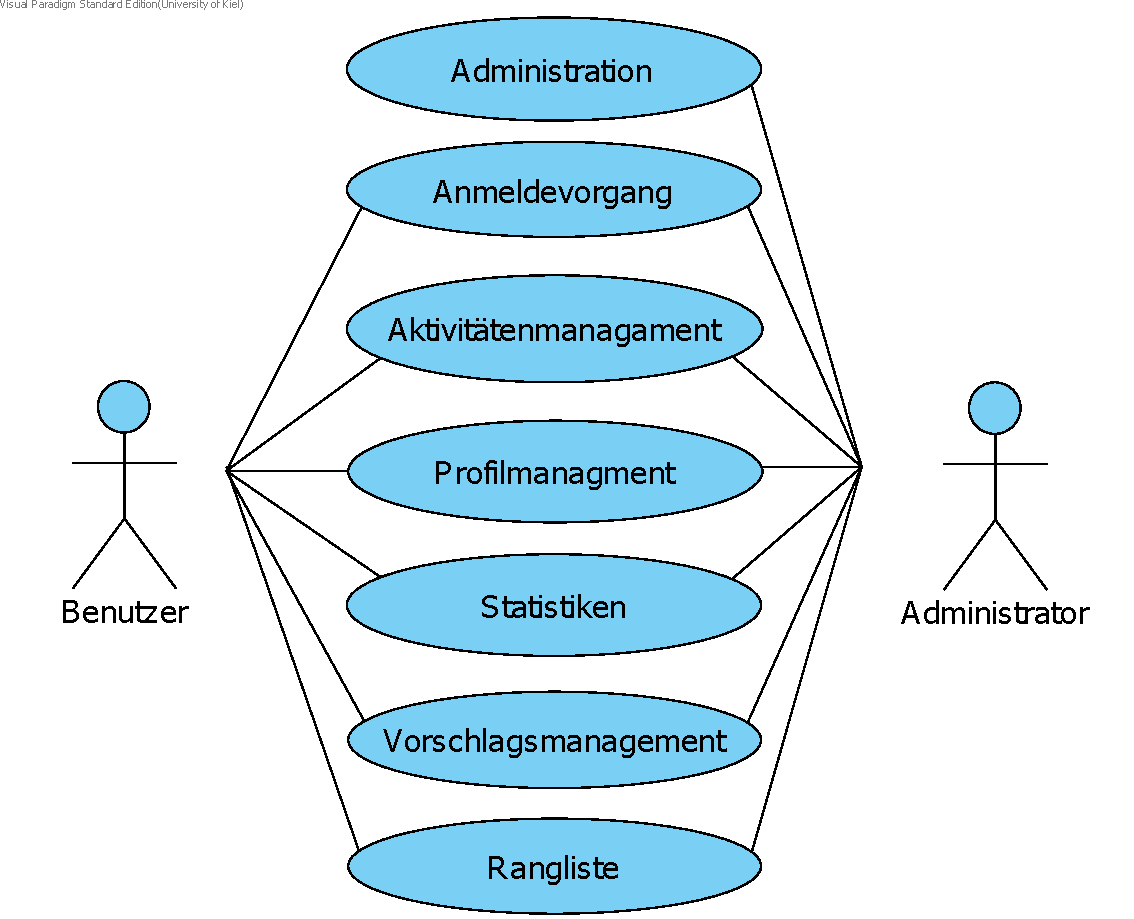
\includegraphics[width=\textwidth]{gfx/Produktuebersicht}
	 \caption{Produkt\"ubersicht}
\end{figure}
%------------------------------------------------
% Akteure
%------------------------------------------------
\section{Akteure}\\
Die folgenden Akteure werden in den beschriebenen Anwendungsfällen benutzt: \\

\begin{tabular}{|p{5cm}|p{5cm}|p{5cm}}
\begin{tabular}{|l|p{.5\linewidth}|}
\hline Akteur & Beschreibung & Verwendet in Anwendungsszenario \\
\hline Benutzer & Ein Benutzer kann sich registrieren, sein Profil bearbeiten, Aktivitäten annehmen und erfüllen, Statistiken und Ranglisten anschauen und Vorschläge unterbreiten oder bewerten & Anmeldevorgang, Aktivitätenmanagement, Profilmanagement, Statistiken, Vorschlagsmanagement, Rangliste \\
\hline Administrator & Ein Administrator ist ein Benutzer mit zusätzlichen Rechten, wie z.B. Profile sperren, löschen oder reaktivieren, Challenges erstellen, bewertete Vorschläge in Aktivitäten umwandeln & Anmeldevorgang, Aktivitätenmanagment, Profilmanagment, Statistiken, Vorschlagsmanagement, Rangliste, Administration\\
\hline

%------------------------------------------------
% Produktfunktion
%------------------------------------------------
\section{Produktfunktion}
\subsection{Webseite}

\subsubsection{Startseite}
	\begin{figure}[H]
	  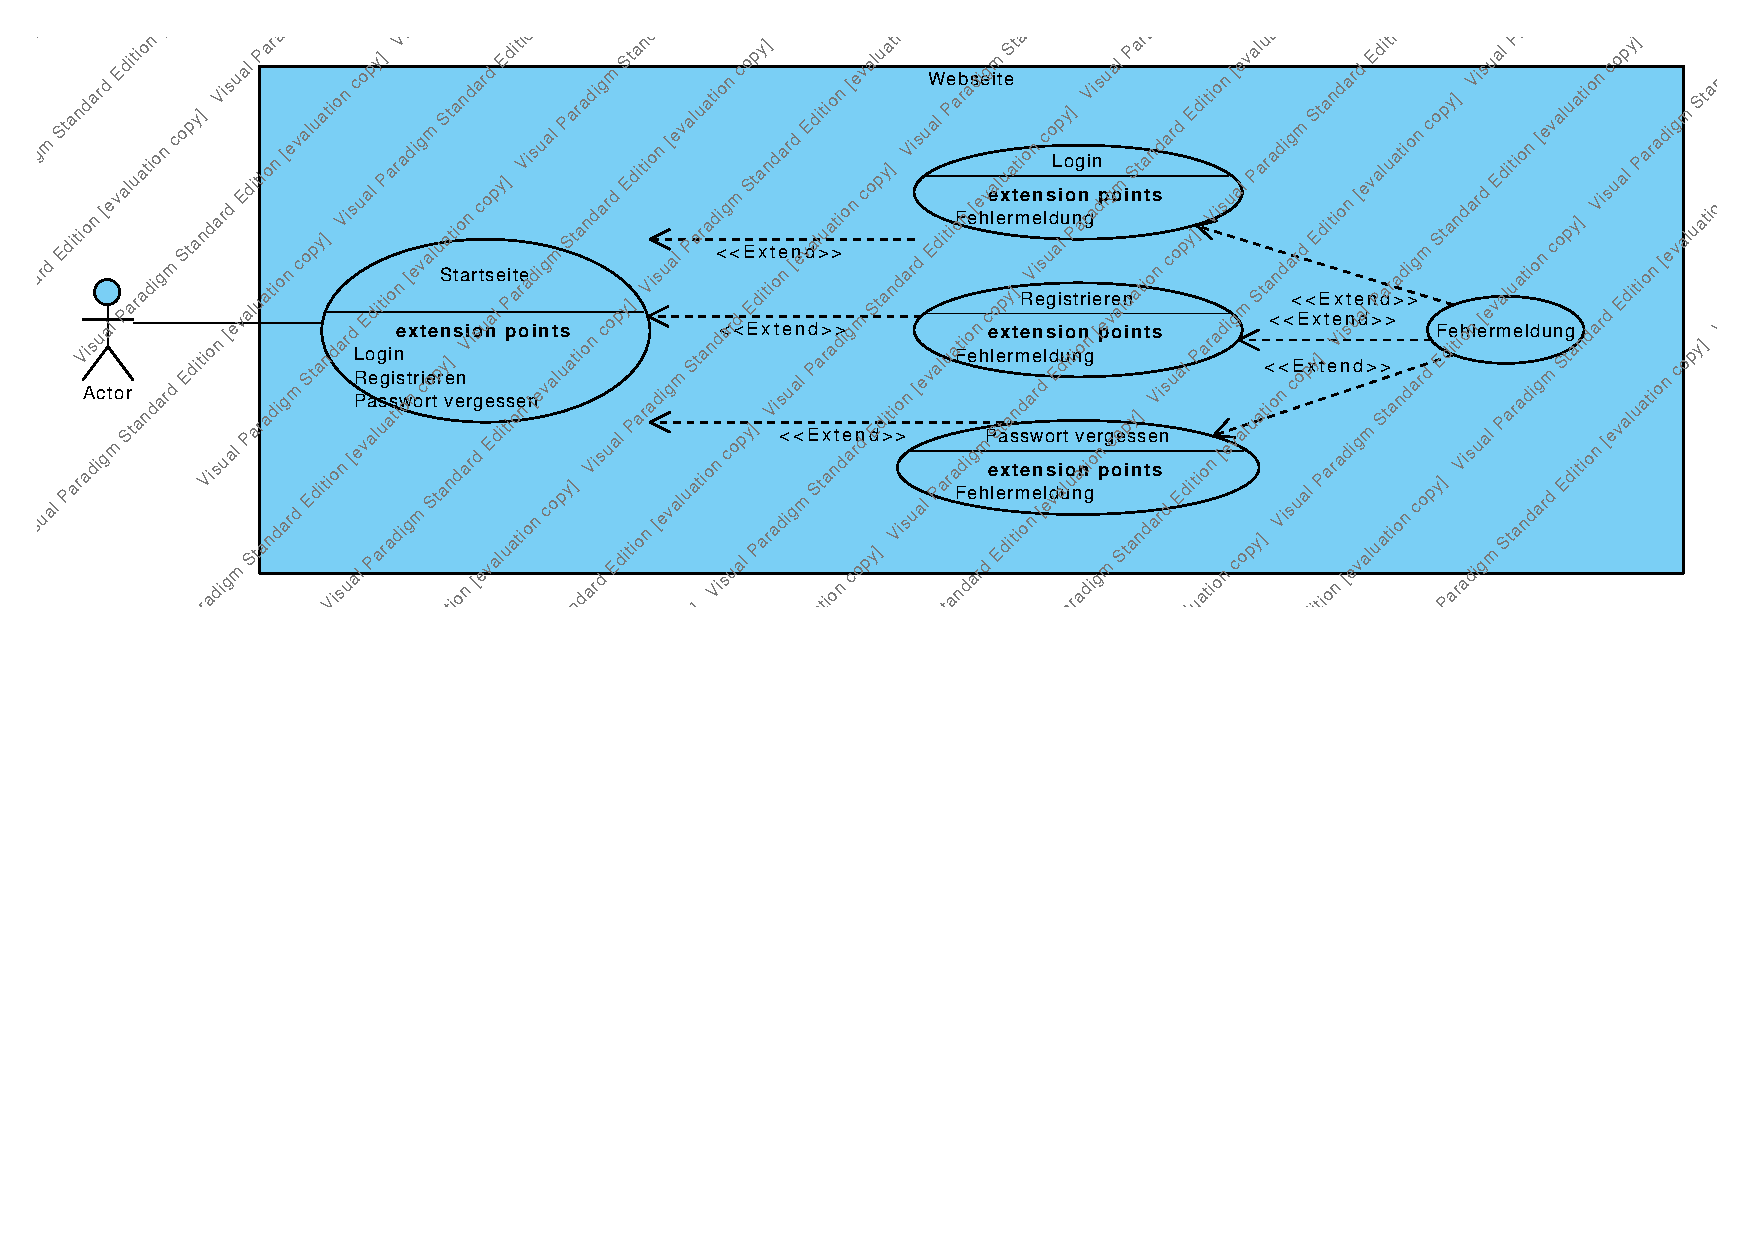
\includegraphics[width=\linewidth]{gfx/webseite/startseite.pdf}
          \caption{Use Case 1.1 Startseite}
	\end{figure}
	\begin{tabularx}{\textwidth}{|l|X|}
	\hline Use Case Nummer & 1.1 \\ 
	\hline Use Case Name & Startseite \\ 
	\hline Initiierender Akteur & Benutzer \\
	\hline Weitere Akteure &  \\
	\hline Kurzbeschreibung & Der Benutzer ruft die Startseite im Browser auf und hat die M\"oglichkeit sich zu registrieren, einzuloggen und das Passwort neu anzufordern. \\
	\hline Vorbedingung & Der Benutzer ist nicht eingeloggt. \\
	\hline Nachbedingung &  \\
	\hline \multicolumn{2}{|c|}{Funktionalität des Use Cases}\\
	\hline Ablauf & Der Benutzer ruft die Webseite auf. \\
	\hline Alternativen &  \\
	\hline Ausnahmen &  \\
	\hline Benutzte Use Cases &  \\
	\hline \multicolumn{2}{|c|}{Weitere Informationen} \\
	\hline Spezielle Anforderungen &  \\
	\hline Annahmen &  \\
	\hline
	\end{tabularx} 
\subsubsection{Login}
	\begin{tabularx}{\textwidth}{|l|X|}
	\hline Use Case Nummer & 1.1.1 \\ 
	\hline Use Case Name & Login \\ 
	\hline Initiierender Akteur & Benutzer \\
	\hline Weitere Akteure & \\
	\hline Kurzbeschreibung & Mit dem Login stehen die eigentlichen Funktionen im Browser zur Verf\"ugung. \\
	\hline Vorbedingung & Der Benutzer ist registriert und nicht eingeloggt. \\
	\hline Nachbedingung & Der Benutzer ist eingeloggt und wurde zu seiner Landingpage weitergeleitet. \\
	\hline \multicolumn{2}{|c|}{Funktionalität des Use Cases}\\
	\hline Ablauf & \begin{itemize}
		\item Der Benutzer gibt seine E-Mail-Adresse und sein Passwort ein.
		\item Der Benutzer klickt den Login Button.
                \item Die Anmeldedaten werden überprüft.
                \item Der Benutzer wird zu seiner Landingpage weitergeleitet.
	\end{itemize} \\
	\hline Alternativen &  \\
	\hline Ausnahmen & \begin{itemize}
		\item Das Passwort ist falsch. Es wird eine Fehlermeldung angezeigt und die Option ``Passwort vergessen'' angeboten.
		\item Die E-Mail-Adresse ist noch nicht registriert. Es wird eine Fehlermeldung angezeigt, und die Registrierung angeboten.
	\end{itemize} \\
	\hline Benutzte Use Cases &  \\
	\hline \multicolumn{2}{|c|}{Weitere Informationen} \\
	\hline Spezielle Anforderungen &  \\
	\hline Annahmen &  \\
	\hline
	\end{tabularx}
			 
\subsubsection{Registrieren}
	\begin{tabularx}{\textwidth}{|l|X|}
	\hline Use Case Nummer & 1.1.2 \\ 
	\hline Use Case Name & Registrieren \\ 
	\hline Initiierender Akteur & Benutzer \\
	\hline Weitere Akteure &  \\
	\hline Kurzbeschreibung & Ein neuer Benutzer kann sich mit seiner E-Mail-Adresse anmelden \\
	\hline Vorbedingung & Benutzer hat auf Registrieren geklickt \\
	\hline Nachbedingung & Benutzer ist eingeloggt \\
	\hline \multicolumn{2}{|c|}{Funktionalität des Use Cases}\\
	\hline Ablauf & \begin{itemize}
		\item Benutzer gibt E-Mail-Adresse und Passwort ein
		\item Benutzer w\"ahlt Fakult\"at
		\item Benutzer klickt "jetzt mitmachen"
	\end{itemize} \\
	\hline Alternativen &  \\
	\hline Ausnahmen & \begin{itemize}
		\item E-Mail-Adresse ist schon vergeben, es wird eine Fehlermeldung angezeigt
		\item das Passwort ist zu kurz, es wird eine Fehlermeldung angezeigt
		\item keine Fakult\"at gewählt, es wird eine Fehlermeldung angezeigt
	\end{itemize} \\
	\hline Benutzte Use Cases &  \\
	\hline \multicolumn{2}{|c|}{Weitere Informationen} \\
	\hline Spezielle Anforderungen &  \\
	\hline Annahmen &  \\
	\hline
	\end{tabularx} 
		
\subsubsection{Passwort vergessen}
	\begin{tabularx}{\textwidth}{|l|X|}
	\hline Use Case Nummer & 1.1.3 \\ 
	\hline Use Case Name & Passwort vergessen \\ 
	\hline Initiierender Akteur & Benutzer \\
	\hline Weitere Akteure &  \\
	\hline Kurzbeschreibung & Ein Benutzer hat die M\"oglichkeit sein Passwort neu per E-Mail anzufordern \\
	\hline Vorbedingung & Benutzer ist nicht eingeloggt \\
	\hline Nachbedingung & Benutzer hat eine E-Mail mit seinem Passwort bekommen \\
	\hline \multicolumn{2}{|c|}{Funktionalität des Use Cases}\\
	\hline Ablauf & \begin{itemize}
		\item Benutzer gibt seine E-Mail-Adresse an.
		\item Benutzer klickt auf ``jetzt Passwort anfordern''.
	\end{itemize} \\
	\hline Alternativen &  \\
	\hline Ausnahmen & E-Mail-Adresse ist nicht registriert, es wird eine Fehlermeldung angezeigt \\
	\hline Benutzte Use Cases &  \\
	\hline \multicolumn{2}{|c|}{Weitere Informationen} \\
	\hline Spezielle Anforderungen &  \\
	\hline Annahmen &  \\
	\hline
\end{tabularx}

\subsubsection{Fehlermeldung} %TODO evtl. später Fehlermeldungen differenzierter betrachten
	\begin{tabularx}{\textwidth}{|l|X|}
	\hline Use Case Nummer & 1.1.4 \\ 
	\hline Use Case Name & Fehlermeldung \\ 
	\hline Initiierender Akteur & Benutzer \\
	\hline Weitere Akteure &  \\
	\hline Kurzbeschreibung & Dem Benutzer wird auf der Startseite eine Fehlermeldung angezeigt \\
	\hline Vorbedingung &  \\
	\hline Nachbedingung & Fehlermeldung wurde angezeigt \\
	\hline \multicolumn{2}{|c|}{Funktionalität des Use Cases}\\
	\hline Ablauf & Fehlermeldung wird auf der Startseite angezeigt. \\
	\hline Alternativen &  \\
	\hline Ausnahmen &  \\
	\hline Benutzte Use Cases &  \\
	\hline \multicolumn{2}{|c|}{Weitere Informationen} \\
	\hline Spezielle Anforderungen &  \\
	\hline Annahmen &  \\
	\hline
	\end{tabularx}
                
%------------------
\subsection{Landingpage}

		\begin{figure}[H]
			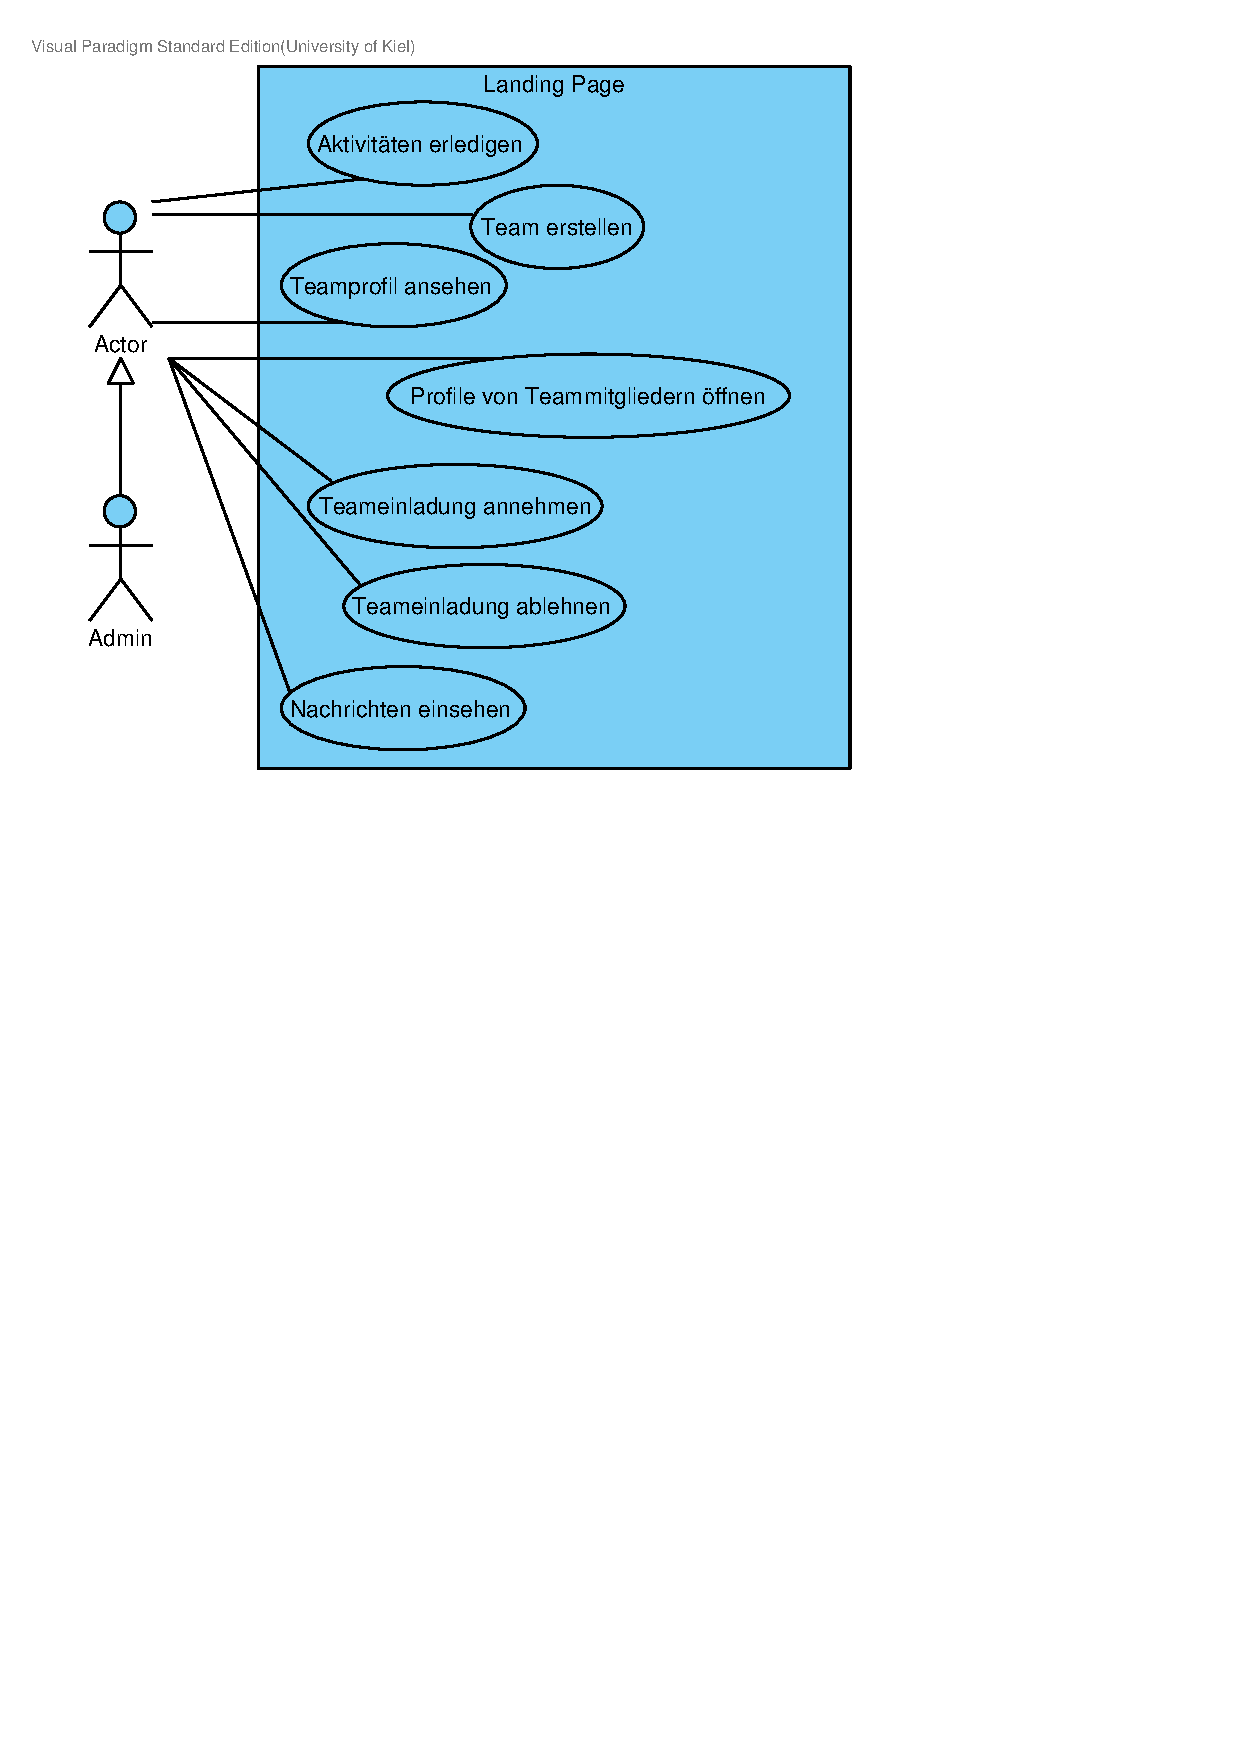
\includegraphics[width=\linewidth]{gfx/webseite/LandingPage.pdf}
			\caption{Use Case 1.2 Landingpage}
		\end{figure}
		\subsubsection{Landingpage}
		\begin{tabularx}{\textwidth}{|l|X|}
			\hline Use Case Nummer & 1.2 \\ 
			\hline Use Case Name & Landingpage \\ 
			\hline Initiierender Akteur & Benutzer \\
			\hline Weitere Akteure &  \\
			\hline Kurzbeschreibung & Die Landingpage ist die Seite direkt nach dem Log-In, auf der der Benutzer Neuigkeiten, seine Teamverwaltung, seine Aktivitäten etc. einsehen kann \\
			\hline Vorbedingung & Der Benutzer ist eingeloggt \\
			\hline Nachbedingung & Der Benutzer befindet sich auf der Landingpage \\
			\hline \multicolumn{2}{|c|}{Funktionalität des Use Cases}\\
			\hline Ablauf & \begin{itemize}
				\item Benutzer loggt sich ein
				\item Benutzer sieht die Landingpage an
			\end{itemize} \\
			\hline Alternativen & \\
			\hline Ausnahmen & \\
			\hline Benutzte Use Cases & \\
			\hline \multicolumn{2}{|c|}{Weitere Informationen} \\
			\hline Spezielle Anforderungen & \\
			\hline Annahmen & \\
			\hline
		\end{tabularx}
		
		\subsubsection{Aktivität erledigen}
		\begin{tabularx}{\textwidth}{|l|X|}
			\hline Use Case Nummer & 1.2.1 \\ 
			\hline Use Case Name & Aktivität erledigen \\ 
			\hline Initiierender Akteur & Benutzer \\
			\hline Weitere Akteure & \\
			\hline Kurzbeschreibung & Der Benutzer kann eine Aktivität als erledigt markieren \\
			\hline Vorbedingung & Der Benutzer befindet sich auf der Landingpage und markiert eine Aktivität als erledigt \\
			\hline Nachbedingung & Die markierte Aktivität wird als erledigt markiert (ausgegraut, je nach Häufigkeitsattribut) \\
			\hline \multicolumn{2}{|c|}{Funktionalität des Use Cases}\\
			\hline Ablauf & \begin{itemize}
				\item Benutzer wählt erledigte Aktivität aus
				\item Aktivität wird als erledigt markiert
			\end{itemize} \\
			\hline Alternativen & \\
			\hline Ausnahmen & \\
			\hline Benutzte Use Cases & \\
			\hline \multicolumn{2}{|c|}{Weitere Informationen} \\
			\hline Spezielle Anforderungen & \\
			\hline Annahmen & \\
			\hline
		\end{tabularx}
		
		\subsubsection{Team erstellen}
		\begin{tabularx}{\textwidth}{|l|X|}
				\hline Use Case Nummer & 1.2.2 \\ 
				\hline Use Case Name & Team erstellen \\ 
				\hline Initiierender Akteur & Benutzer \\
				\hline Weitere Akteure & \\
				\hline Kurzbeschreibung & Der Benutzer kann über die entsprechende Schaltfläche ein neues Team erstellen \\
				\hline Vorbedingung & Der Benutzer ist eingeloggt und befindet sich auf der Landingpage \\
				\hline Nachbedingung & Das auszufüllende Formular für ein Teamprofil wird angezeigt \\
				\hline \multicolumn{2}{|c|}{Funktionalität des Use Cases}\\
				\hline Ablauf & \begin{itemize}
					\item Benutzer klickt auf Team erstellen
					\item Teamprofil Formular wird angezeigt
					\item Team wird den eigenen Teams hinzugefügt
				\end{itemize} \\
				\hline Alternativen & \\
				\hline Ausnahmen & \\
				\hline Benutzte Use Cases & \\
				\hline \multicolumn{2}{|c|}{Weitere Informationen} \\
				\hline Spezielle Anforderungen & \\
				\hline Annahmen & \\
				\hline
		\end{tabularx}
			
		\subsubsection{Teameinladung annehmen}		
		\begin{tabularx}{\textwidth}{|l|X|}
			\hline Use Case Nummer & 1.2.3 \\ 
			\hline Use Case Name & Teameinladung annehmen \\ 
			\hline Initiierender Akteur & Benutzer \\
			\hline Weitere Akteure & \\
			\hline Kurzbeschreibung & Der Benutzer kann Teameinladungen von anderen Benutzern annehmen \\
			\hline Vorbedingung & Der Benutzer befindet sich auf der Landingpage \\
			\hline Nachbedingung & Die Einladung ist aus der Teamübersicht verschwunden und das Team nun bei den Teams des Benutzers aufgeführt \\
			\hline \multicolumn{2}{|c|}{Funktionalität des Use Cases}\\
			\hline Ablauf & \begin{itemize}
				\item Benutzer akzeptiert die Teameinladung in der Teamübersicht
				\item Benutzer ist Mitglied des Teams und das Team wird in seiner Teamübersicht angezeigt
			\end{itemize} \\
			\hline Alternativen & \\
			\hline Ausnahmen & \\
			\hline Benutzte Use Cases & \\
			\hline \multicolumn{2}{|c|}{Weitere Informationen} \\
			\hline Spezielle Anforderungen & \\
			\hline Annahmen & \\
			\hline
		\end{tabularx}
			
		\subsubsection{Teameinladung ablehnen}
		\begin{tabularx}{\textwidth}{|l|X|}
			\hline Use Case Nummer & 1.2.4 \\ 
			\hline Use Case Name & Teameinladung ablehnen \\ 
			\hline Initiierender Akteur & Benutzer \\
			\hline Weitere Akteure & \\
			\hline Kurzbeschreibung & Der Benutzer kann eine Einladung einem Team beizutreten ablehnen \\
			\hline Vorbedingung & Der Benutzer ist eingeloggt und befindet sich auf der Landingpage \\
			\hline Nachbedingung & Die Teameinladung ist auf der Landingpage nicht mehr vorhanden \\
			\hline \multicolumn{2}{|c|}{Funktionalität des Use Cases}\\
			\hline Ablauf & \begin{itemize}
				\item Benutzer lehnt die Teameinladung ab
				\item Teameinladung wird aus Teamübersicht gelöscht
			\end{itemize} \\
			\hline Alternativen & \\
			\hline Ausnahmen & \\
			\hline Benutzte Use Cases & \\
			\hline \multicolumn{2}{|c|}{Weitere Informationen} \\
			\hline Spezielle Anforderungen & \\
			\hline Annahmen & \\
			\hline
		\end{tabularx}
				
		\subsubsection{Teamprofil ansehen}
		\begin{tabularx}{\textwidth}{|l|X|}
			\hline Use Case Nummer & 1.2.5 \\ 
			\hline Use Case Name & Teamprofil ansehen \\ 
			\hline Initiierender Akteur & Benutzer \\
			\hline Weitere Akteure & \\
			\hline Kurzbeschreibung & Der Benutzer kann durch Anklicken eines Teamnamens oder -fotos das Profil des entsprechenden Teams aufrufen \\
			\hline Vorbedingung & Der Benutzer befindet sich auf der Landingpage und ist Mitglied eines Teams bzw. hat eine Teameinladung vorliegen \\
			\hline Nachbedingung & Die Teamprofil-Ansicht ist geöffnet \\
			\hline \multicolumn{2}{|c|}{Funktionalität des Use Cases}\\
			\hline Ablauf & \begin{itemize}
				\item Benutzer klickt Teamname oder -bild an
				\item Benutzer wird auf Teamprofil geleitet
			\end{itemize} \\
			\hline Alternativen & \\
			\hline Ausnahmen & \\
			\hline Benutzte Use Cases & \\
			\hline \multicolumn{2}{|c|}{Weitere Informationen} \\
			\hline Spezielle Anforderungen & \\
			\hline Annahmen & \\
			\hline
		\end{tabularx}
				
		\subsubsection{Profil von Teammitglied ansehen}
		\begin{tabularx}{\textwidth}{|l|X|}
			\hline Use Case Nummer & 1.2.6 \\ 
			\hline Use Case Name & Profil von Teammitglied ansehen \\ 
			\hline Initiierender Akteur & Benutzer \\
			\hline Weitere Akteure & \\
			\hline Kurzbeschreibung & Der Benutzer kann sich die Profile seiner Teammitglieder ansehen \\
			\hline Vorbedingung & Der Benutzer ist Mitglied eines Teams und befindet sich auf der Landingpage \\
			\hline Nachbedingung & Der Benutzer befindet sich auf der Profilseite des ausgewählten Teammitglieds \\
			\hline \multicolumn{2}{|c|}{Funktionalität des Use Cases}\\
			\hline Ablauf & \begin{itemize}
				\item Benutzer klickt den Namen eines Teammitglieds an
				\item Benutzer wird auf die Profilseite des Teammitglieds weitergeleitet
			\end{itemize} \\
			\hline Alternativen & \\
			\hline Ausnahmen & \\
			\hline Benutzte Use Cases & \\
			\hline \multicolumn{2}{|c|}{Weitere Informationen} \\
			\hline Spezielle Anforderungen & \\
			\hline Annahmen & \\
			\hline
		\end{tabularx}
					
		\subsubsection{Nachrichten einsehen}
		\begin{tabularx}{\textwidth}{|l|X|}
			\hline Use Case Nummer & 1.2.7 \\ 
			\hline Use Case Name & Nachrichten einsehen \\ 
			\hline Initiierender Akteur & Benutzer \\
			\hline Weitere Akteure & \\
			\hline Kurzbeschreibung & Der Benutzer kann die zuletzt von Teammitgliedern erledigten Aktivitäten / Challenges über ein Benachrichtigungsymbol in einem PopUp ansehen \\
			\hline Vorbedingung & Der Benutzer befindet sich auf der Landingpage \\
			\hline Nachbedingung & Der Benutzer befindet sich auf der Landingpage und ein PopUp öffnet sich, in welchem die Nachricht enthalten ist \\
			\hline \multicolumn{2}{|c|}{Funktionalität des Use Cases}\\
			\hline Ablauf & \\
			\hline Alternativen & Es sind noch keine Nachrichten vorhanden, da der Benutzer kein Mitglied eines Teams ist \\
			\hline Ausnahmen & \\
			\hline Benutzte Use Cases & \\
			\hline \multicolumn{2}{|c|}{Weitere Informationen} \\
			\hline Spezielle Anforderungen & \\
			\hline Annahmen & \\
			\hline
		\end{tabularx}
%-----------------
\subsection{Aktivit\"aten}

	\begin{figure}[H]
		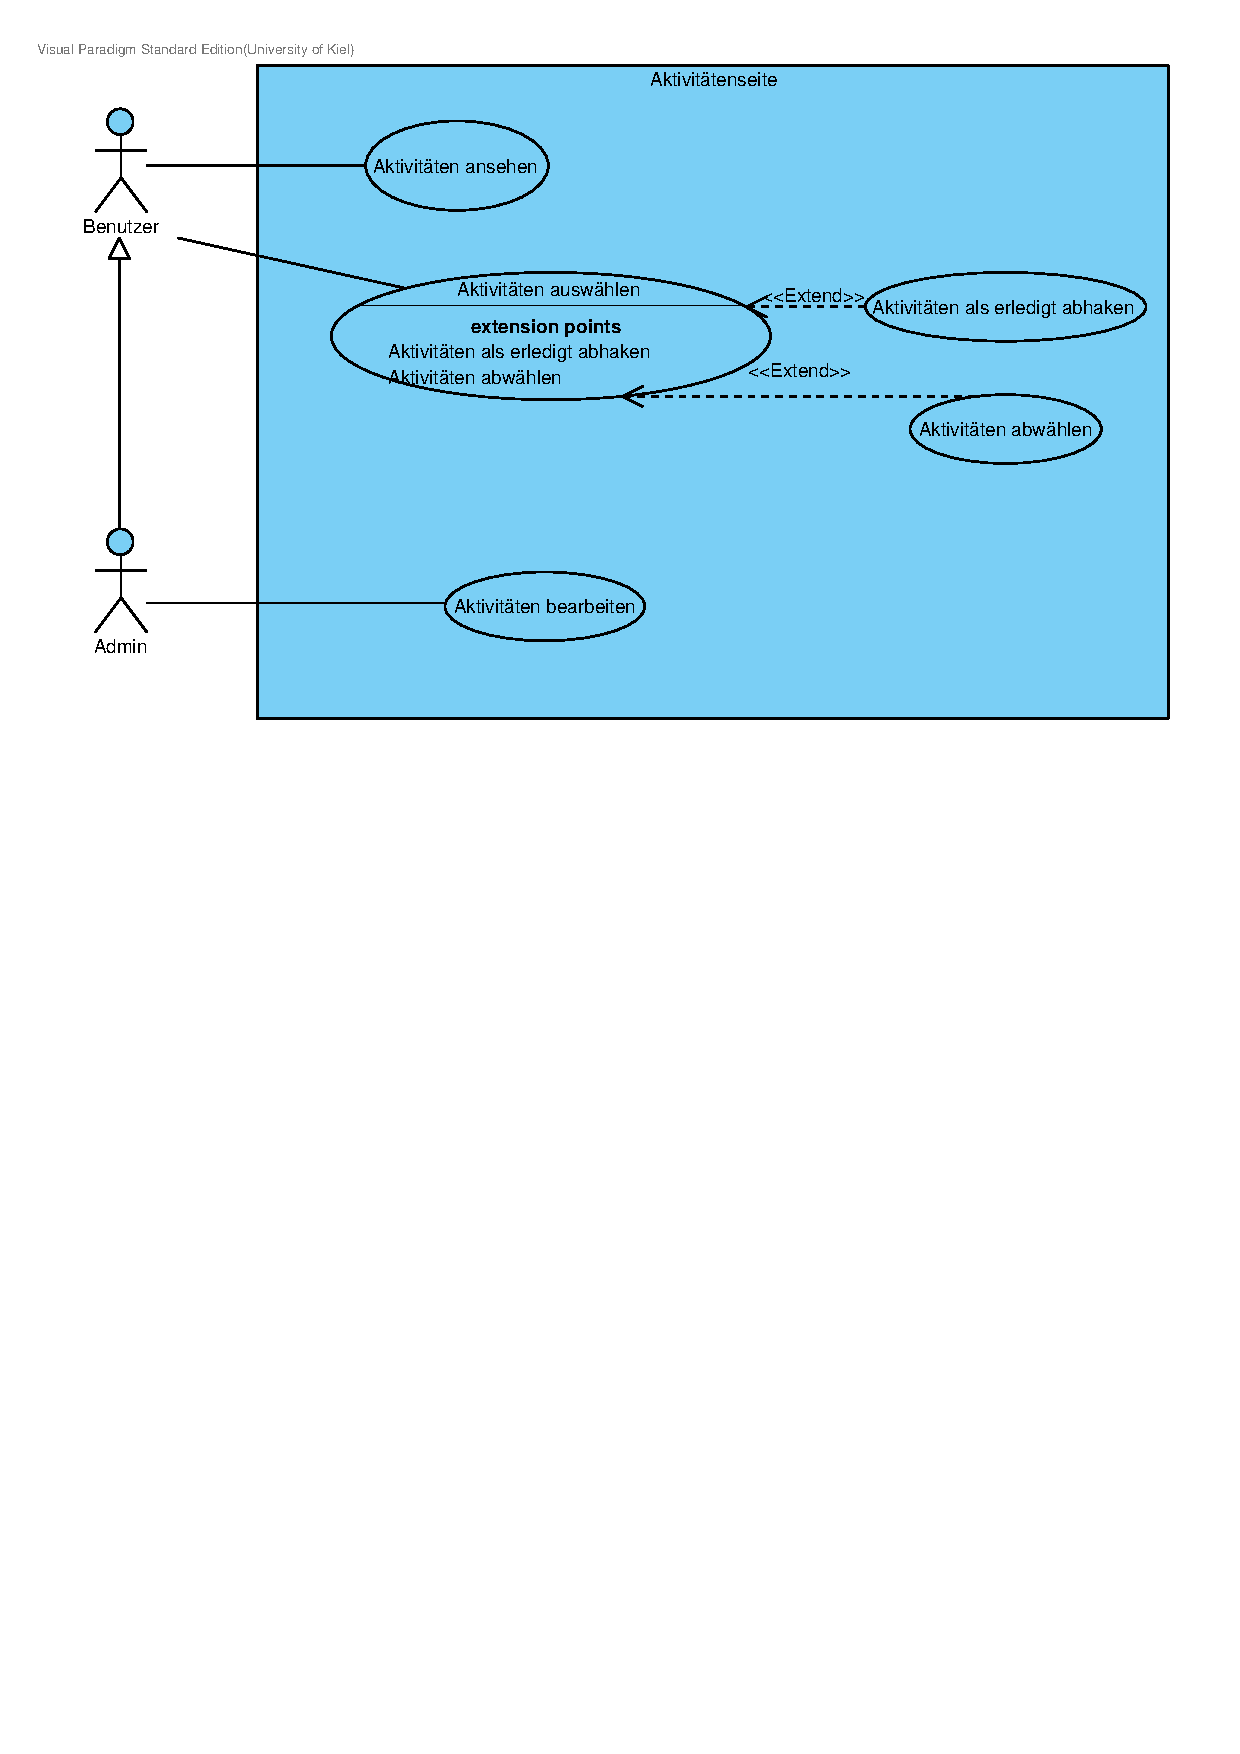
\includegraphics[width=\linewidth]{gfx/webseite/Aktivitaetenseite.pdf}
		\caption{Use Case 1.3 Aktivit\"aten}
	\end{figure}
	\subsubsection{Aktivit\"atenseite}
	\begin{tabularx}{\textwidth}{|l|X|}
	\hline Use Case Nummer & 1.3 \\ 
	\hline Use Case Name & Aktivit\"atenseite \\ 
	\hline Initiierender Akteur & Benutzer \\
	\hline Weitere Akteure & \\
	\hline Kurzbeschreibung & Der Benutzer kann eine Liste von verf\"ugbaren Aktivit\"aten ansehen, sowie Aktivit\"aten favorisieren oder als erledigt markieren \\
	\hline Vorbedingung & Die Aktivit\"atenseite ist im Browser aufgerufen \\
	\hline Nachbedingung & Die Aktivit\"atenseite ist im Browser aufgerufen \\
	\hline \multicolumn{2}{|c|}{Funktionalität des Use Cases}\\
	\hline Ablauf & Benutzer ruft die Aktivit\"atenseite auf \\
	\hline Alternativen & \\
	\hline Ausnahmen & Die Aktivit\"atenseite ist nicht verf\"ugbar \\
	\hline Benutzte Use Cases & \\
	\hline \multicolumn{2}{|c|}{Weitere Informationen} \\
	\hline Spezielle Anforderungen & \\
	\hline Annahmen & \\
	\hline
	\end{tabularx} 
	\subsubsection{Aktivit\"aten ansehen}
	\begin{tabularx}{\textwidth}{|l|X|}
	\hline Use Case Nummer & 1.3.1 \\ 
	\hline Use Case Name & Aktivit\"aten ansehen \\ 
	\hline Initiierender Akteur & Benutzer \\
	\hline Weitere Akteure & \\
	\hline Kurzbeschreibung & Der Benutzer kann die auf der Seite dargestellte Liste von verf\"ugbaren Aktivit\"aten einsehen \\
	\hline Vorbedingung & Die Aktivit\"atenseite ist im Browser aufgerufen \\
	\hline Nachbedingung & Die Aktivit\"atenseite ist im Browser aufgerufen \\
	\hline \multicolumn{2}{|c|}{Funktionalität des Use Cases}\\
	\hline Ablauf & Der Benutzer sieht die Liste der Aktivit\"aten an \\
	\hline Alternativen & \\
	\hline Ausnahmen & Die Aktivit\"atenliste ist nicht verf\"ugbar \\
	\hline Benutzte Use Cases & \\
	\hline \multicolumn{2}{|c|}{Weitere Informationen} \\
	\hline Spezielle Anforderungen & \\
	\hline Annahmen & \\
	\hline
	\end{tabularx} 
	\subsubsection{Aktivit\"aten erledigen}
	\begin{tabularx}{\textwidth}{|l|X|}
	\hline Use Case Nummer & 1.3.2\\ 
	\hline Use Case Name & Aktivit\"aten erledigen \\ 
	\hline Initiierender Akteur & Benutzer \\
	\hline Weitere Akteure & \\
	\hline Kurzbeschreibung & Der Benutzer kann Aktivit\"aten erledigen \\
	\hline Vorbedingung & Der Benutzer befindet sich auf der Aktivit\"atenseite \\
	\hline Nachbedingung & Die abgeschlossene/n Aktivit\"at/en werden als solche markiert und dem Benutzer die entsprechende Punktzahl gutgeschrieben \\
	\hline \multicolumn{2}{|c|}{Funktionalität des Use Cases}\\
	\hline Ablauf & \begin{itemize}
			\item Benutzer klicken auf die Aktivit\"at
			\item Die Aktivit\"at wird als erledigt markiert und dem Benutzer die entsprechenden Punkte gutgeschrieben
		\end{itemize} \\
	\hline Alternativen & \\
	\hline Ausnahmen & Die Aktivit\"at ist in dem Zeitraum bzw. derzeit nicht verf\"ugbar \\
	\hline Benutzte Use Cases &  \\
	\hline \multicolumn{2}{|c|}{Weitere Informationen} \\
	\hline Spezielle Anforderungen & \\
	\hline Annahmen & \\
	\hline
	\end{tabularx} 
	\subsubsection{Aktivit\"aten favorisieren}
	\begin{tabularx}{\textwidth}{|l|X|}
	\hline Use Case Nummer & 1.3.3 \\ 
	\hline Use Case Name & Aktivit\"aten favorisieren \\ 
	\hline Initiierender Akteur & Benutzer \\
	\hline Weitere Akteure & \\
	\hline Kurzbeschreibung & Der Benutzer kann eine oder mehrere Aktivit\"aten favorisieren \\
	\hline Vorbedingung & Der Benutzer befindet sich auf der Aktivit\"atenseite \\
	\hline Nachbedingung & Die favorisierten Aktivit\"aten erscheinen auf der Landingpage und auf werden außerdem auf der Aktivit\"atenseite als favorisiert angezeigt \\
	\hline \multicolumn{2}{|c|}{Funktionalität des Use Cases}\\
	\hline Ablauf & Benutzer favorisiert über einen Button eine oder mehrere der Aktivit\"aten \\
	\hline Alternativen & \\
	\hline Ausnahmen & Die Aktivit\"atenliste ist nicht verf\"ugbar \\
	\hline Benutzte Use Cases & \\
	\hline \multicolumn{2}{|c|}{Weitere Informationen} \\
	\hline Spezielle Anforderungen & \\
	\hline Annahmen & \\
	\hline
	\end{tabularx} 
	\subsubsection{Aktivit\"aten bearbeiten}
	\begin{tabularx}{\textwidth}{|l|X|}
	\hline Use Case Nummer & 1.3.4 \\ 
	\hline Use Case Name & Aktivit\"aten bearbeiten \\ 
	\hline Initiierender Akteur & Admin \\
	\hline Weitere Akteure & \\
	\hline Kurzbeschreibung & Der Admin kann einzelne Aktivit\"aten bearbeiten (Name, Punktzahl, Zeitraum, etc.) \\
	\hline Vorbedingung & Die Aktivit\"atenseite ist im Browser aufgerufen und eine Aktivit\"at zur Bearbeitung ausgew\"ahlt \\
	\hline Nachbedingung & Die bearbeitete Aktivit\"at wird in ihrer neuen Form in der Aktivit\"atenliste angezeigt \\
	\hline \multicolumn{2}{|c|}{Funktionalität des Use Cases}\\
	\hline Ablauf & \begin{itemize}
			\item Der Admin w\"ahlt eine Aktivit\"at zur Bearbeitung aus
			\item Der Admin speichert die Aktivit\"at mit den vorgenommenen \"Anderungen
		\end{itemize} \\
	\hline Alternativen & Der Admin l\"oscht die Aktivit\"at \\
	\hline Ausnahmen & Die Aktivit\"atenliste ist nicht verf\"ugbar \\
	\hline Benutzte Use Cases & 1.3.1 Aktivit\"aten ansehen \\
	\hline \multicolumn{2}{|c|}{Weitere Informationen} \\
	\hline Spezielle Anforderungen & \\
	\hline Annahmen & \\
	\hline
	\end{tabularx} 

\subsection{Energiespavorschl\"age}

\begin{tabularx}{\textwidth}{|l|X|}
		\hline Use Case Nummer & 1.4\\ 
		\hline Use Case Name & Vorschlagsseite \\ 
		\hline Initiierender Akteur & Benutzer \\
		\hline Weitere Akteure & \\
		\hline Kurzbeschreibung & Die Vorschlagsseite ist dafür, dass Benutzer Vorschl\"age für neue Aktivit\"aten abgeben, bewerten und kommentieren k\"onnen. Der Admin kann hier Vorschl\"age in Aktivit\"aten umwandeln.\\
		\hline Vorbedingung & Der Benutzer ist eingeloggt und befindet sich auf der Vorschlagsseite \\
		\hline Nachbedingung & Der Benutzer befindet sich auf der Vorschlagsseite \\
		\hline \multicolumn{2}{|c|}{Funktionalität des Use Cases}\\
		\hline Ablauf & Der Benutzer/Admin ruft die Vorschlagsseite auf \\
		\hline Alternativen & \\
		\hline Ausnahmen & \\
		\hline Benutzte Use Cases & \\
		\hline \multicolumn{2}{|c|}{Weitere Informationen} \\
		\hline Spezielle Anforderungen & \\
		\hline Annahmen & \\
		\hline
	\end{tabularx}

	\subsubsection{Vorschlagsliste ansehen}
	\begin{tabularx}{\textwidth}{|l|X|}
		\hline Use Case Nummer & 1.4.1 \\ 
		\hline Use Case Name & Vorschlagsliste ansehen \\ 
		\hline Initiierender Akteur & Benutzer \\
		\hline Weitere Akteure & \\
		\hline Kurzbeschreibung & Der Benutzer kann die auf der Seite dargestellte Liste von verf\"ugbaren Vorschl\"age einsehen \\
		\hline Vorbedingung & Die Vorschlagsseite ist im Browser aufgerufen \\
		\hline Nachbedingung & Die Vorschlagsseite ist im Browser aufgerufen \\
		\hline \multicolumn{2}{|c|}{Funktionalität des Use Cases}\\
		\hline Ablauf & Der Benutzer sieht die Liste der Vorschl\"age an\\
		\hline Alternativen &  \\
		\hline Ausnahmen & Die Vorschlagsliste ist nicht verf\"ugbar \\
		\hline Benutzte Use Cases & \\
		\hline \multicolumn{2}{|c|}{Weitere Informationen} \\
		\hline Spezielle Anforderungen &  \\
		\hline Annahmen &  \\
		\hline
	\end{tabularx}	
	
	\subsubsection{Vorschl\"age bewerten}
	\begin{tabularx}{\textwidth}{|l|X|}
		\hline Use Case Nummer & 1.4.1.1 \\ 
		\hline Use Case Name & Vorschl\"age bewerten \\ 
		\hline Initiierender Akteur & Benutzer \\
		\hline Weitere Akteure & \\
		\hline Kurzbeschreibung & Der Benutzer bewertet Vorschl\"age mit Hilfe von Sternen. \\
		\hline Vorbedingung & Der Benutzer hat sich einen Vorschlag angesehen. \\
		\hline Nachbedingung & Die Gesamtbewertung des Vorschlages erscheint aktualisiert neben dem Vorschlag. \\
		\hline \multicolumn{2}{|c|}{Funktionalität des Use Cases}\\
		\hline Ablauf & \begin{itemize}
			\item Der Benutzer bewertet mit Hilfe einer Skala aus Sternen.
			\item Die durschnittliche Bewertung des Vorschlages wird dem Benutzer angezeigt.
		\end{itemize} \\
		\hline Alternativen &  \\
		\hline Ausnahmen &  \\
		\hline Benutzte Use Cases & 1.4.1 Vorschlagsliste ansehen \\
		\hline \multicolumn{2}{|c|}{Weitere Informationen} \\
		\hline Spezielle Anforderungen &  \\
		\hline Annahmen &  \\
		\hline
	\end{tabularx}
	
	\subsubsection{Vorschl\"age kommentieren}
	\begin{tabularx}{\textwidth}{|l|X|}
		\hline Use Case Nummer & 1.4.1.2 \\ 
		\hline Use Case Name & Vorschl\"age kommentieren \\ 
		\hline Initiierender Akteur & Benutzer \\
		\hline Weitere Akteure & \\
		\hline Kurzbeschreibung & Der Benutzer kommentiert einen Vorschlag. \\
		\hline Vorbedingung & Der Benutzer hat sich einen Vorschlag angesehen \\
		\hline Nachbedingung & Der Kommentar wird neben dem Vorschlag angezeigt \\
		\hline \multicolumn{2}{|c|}{Funktionalität des Use Cases}\\
		\hline Ablauf & \begin{itemize}
			\item Der Benutzer schreibt einen Kommentar.
			\item Der Benutzer \"ubermittelt den Kommentar.
			\item Der neue Kommentar wird angezeigt.
		\end{itemize} \\ 
		\hline Alternativen &  \\
		\hline Ausnahmen & \begin{itemize}
			\item Wenn kein Text eingegeben wird, kann der Kommentar nicht \"ubermittelt werden.
			\item Ist der Kommentar zu lang, dann wird er nicht akzeptiert.
		\end{itemize} \\
		\hline Benutzte Use Cases & 1.4.1 Vorschl\"age ansehen\\
		\hline \multicolumn{2}{|c|}{Weitere Informationen} \\
		\hline Spezielle Anforderungen &  \\
		\hline Annahmen &  \\
		\hline
	\end{tabularx}
	
	\subsubsection{Vorschl\"age zu Aktivit\"aten \"andern}
	\begin{tabularx}{\textwidth}{|l|X|}
		\hline Use Case Nummer & 1.4.1.3 \\ 
		\hline Use Case Name & Vorschl\"age zu Aktivit\"aten \"andern \\ 
		\hline Initiierender Akteur & Admin \\
		\hline Weitere Akteure & \\
		\hline Kurzbeschreibung & Der Admin kann über einen Button einen Vorschlag zu einer Aktivit\"at machen und diesen währenddessen editieren. \\
		\hline Vorbedingung & Der Admin hat sich einen Vorschlag angesehen \\
		\hline Nachbedingung & Ein Bearbeitungsfeld zur Editierung öffnet sich\\
		\hline \multicolumn{2}{|c|}{Funktionalität des Use Cases}\\
		\hline Ablauf & \begin{itemize}
			\item Der Admin wählt über einen Button einen Vorschlag aus der Vorschlagsliste aus.
			\item Der Admin editiert auf einem Bearbeitungsfeld den Vorschlag.
			\item Der Admin bestätigt die Editierung und wandelt so den Vorschlag zur Aktivit\"at.
		\end{itemize} \\
		\hline Alternativen &  \\
		\hline Ausnahmen & Die Vorschlagsliste ist nicht verf\"ugbar \\
		\hline Benutzte Use Cases & 1.4.1 Vorschl\"age ansehen \\
		\hline \multicolumn{2}{|c|}{Weitere Informationen} \\
		\hline Spezielle Anforderungen &  \\
		\hline Annahmen &  \\
		\hline
	\end{tabularx}

	\subsubsection{Vorschl\"age erstellen}
	\begin{tabularx}{\textwidth}{|l|X|}
		\hline Use Case Nummer & 1.4.2 \\ 
		\hline Use Case Name & Vorschl\"age erstellen \\ 
		\hline Initiierender Akteur & Benutzer \\
		\hline Weitere Akteure & \\
		\hline Kurzbeschreibung & Der Benutzer gibt in einem Textfeld einen Vorschlag für eine neue Aktivit\"at ein und bestätigt diesen. \\
		\hline Vorbedingung & Ist als Benutzer eingeloggt und auf der Vorschlagsseite \\
		\hline Nachbedingung & Der Benutzer ist auf der Vorschlagsseite und der neue Vorschlag wird angezeigt \\
		\hline \multicolumn{2}{|c|}{Funktionalität des Use Cases}\\
		\hline Ablauf & \begin{itemize}
			\item Der Benutzer/Admin gibt seinen Vorschlag ein (Name der Aktivität, welcher selbst erklärend ist, Punkte, Zeitraum)
			\item Der Benutzer/Admin \"ubermittelt den Vorschlag, welcher anschließend einsehbar ist.
		\end{itemize} \\
		\hline Alternativen &  \\
		\hline Ausnahmen & \begin{itemize}
			\item Wenn eine der erforderlichen Information fehlt, wird der Vorschlag nicht \"ubermittelt.
			\item Wenn die vorgeschlagenen Punktzahl keine ganze Zahl ist, wird der Vorschlag abgelehnt.
			\item Wenn der Zeitraum ungültig ist, wird der Vorschlag abgelehnt.
		\end{itemize} \\
		\hline Benutzte Use Cases &  \\
		\hline \multicolumn{2}{|c|}{Weitere Informationen} \\
		\hline Spezielle Anforderungen &  \\
		\hline Annahmen &  \\
		\hline
	\end{tabularx}
        
%---------------------------------------------
\subsection{Rangliste}
	\begin{figure}[H]
		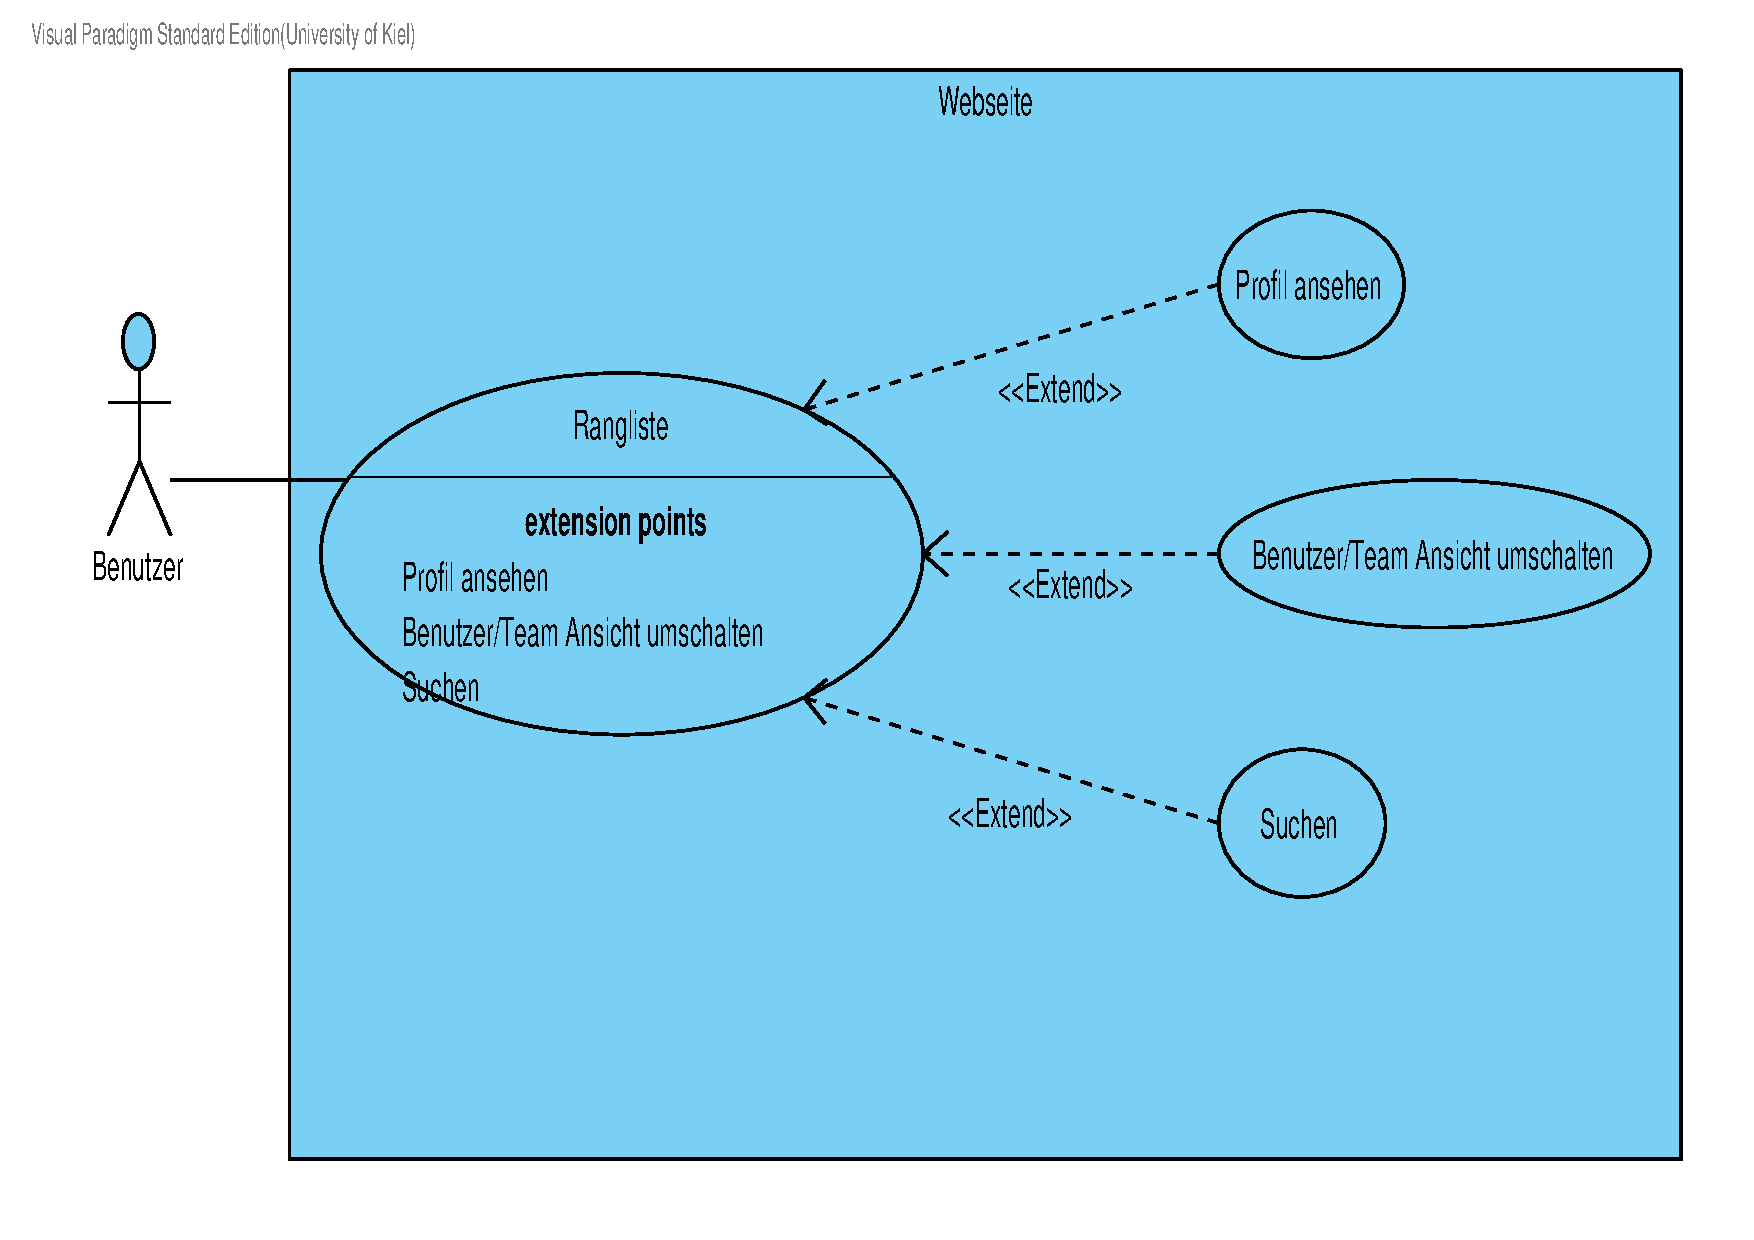
\includegraphics[width=\linewidth]{gfx/webseite/rangliste.pdf}
                \caption{Use Case 1.5 Rangliste ansehen}
        \end{figure}

\subsubsection{Rangliste Ansehen}
	\begin{tabularx}{\textwidth}{|l|X|}
	\hline Use Case Nummer & 1.5 \\ 
	\hline Use Case Name & Rangliste ansehen \\ 
	\hline Initiierender Akteur & Benutzer \\
	\hline Weitere Akteure &  \\
	\hline Kurzbeschreibung & Der Benutzer kann die Rangliste ansehen. \\
	\hline Vorbedingung & Der Benutzer ist eingeloggt. \\
	\hline Nachbedingung & Die Rangliste wird angezeigt. \\
	\hline \multicolumn{2}{|c|}{Funktionalität des Use Cases}\\
	\hline Ablauf & \begin{itemize}
                \item Der Benutzer klickt auf ``Rangliste''. 
                \item Die Rangliste wird angezeigt.
                \end{itemize}\\
	\hline Alternativen & \\
	\hline Ausnahmen &  \\
	\hline Benutzte Use Cases &  \\
	\hline \multicolumn{2}{|c|}{Weitere Informationen} \\
	\hline Spezielle Anforderungen &  \\
	\hline Annahmen &  \\
	\hline
	\end{tabularx}
        
\subsubsection{Profil ansehen}
	\begin{tabularx}{\textwidth}{|l|X|}
	\hline Use Case Nummer & 1.5.1 \\ 
	\hline Use Case Name & Profil ansehen \\ 
	\hline Initiierender Akteur & Benutzer \\
	\hline Weitere Akteure &  \\
	\hline Kurzbeschreibung & Eine Ansicht eines Profils von einem Team oder einem Benutzer ansehen. \\
	\hline Vorbedingung & Es wurde ein Profil angeklickt. \\
	\hline Nachbedingung & Das Profil wird angezeigt. \\
	\hline \multicolumn{2}{|c|}{Funktionalität des Use Cases}\\
	\hline Ablauf & \begin{itemize}
		\item Der Benutzer klickt auf ein Profil.
		\item Das Profil wird angezeigt.
	\end{itemize} \\
	\hline Alternativen &  \\
	\hline Ausnahmen &  \\
	\hline Benutzte Use Cases &  \\
	\hline \multicolumn{2}{|c|}{Weitere Informationen} \\
	\hline Spezielle Anforderungen &  \\
	\hline Annahmen &  \\
	\hline
	\end{tabularx}

\subsubsection{Benutzer/Team Ansicht wechseln}
	\begin{tabularx}{\textwidth}{|l|X|}
	\hline Use Case Nummer & 1.5.2 \\ 
	\hline Use Case Name & Benutzer/Team Ansicht wechseln \\ 
	\hline Initiierender Akteur & Benutzer \\
	\hline Weitere Akteure &  \\
	\hline Kurzbeschreibung & Der Benutzer kann zwischen der Benutzer Ranglite und der Team Rangliste hin und her schalten \\
	\hline Vorbedingung & Rangliste wird angezeigt \\
	\hline Nachbedingung & Ansicht wurde umgeschaltet \\
	\hline \multicolumn{2}{|c|}{Funktionalität des Use Cases}\\
	\hline Ablauf & \begin{itemize}
		\item Benutzer klickt auf "Team"
		\item Team Ansicht wird angezeigt
	\end{itemize} \\
	\hline Alternativen & \begin{itemize}
				\item Benutzer klickt auf "Benutzer"
				\item Benutzer Ansicht wird angezeigt
			\end{itemize} \\
	\hline Ausnahmen &  \\
	\hline Benutzte Use Cases &  \\
	\hline \multicolumn{2}{|c|}{Weitere Informationen} \\
	\hline Spezielle Anforderungen &  \\
	\hline Annahmen &  \\
	\hline
	\end{tabularx}
		
\subsubsection{Suche}
	\begin{tabularx}{\textwidth}{|l|X|}
	\hline Use Case Nummer & 1.5.3 \\ 
	\hline Use Case Name & Suche \\ 
	\hline Initiierender Akteur & Benutzer \\
	\hline Weitere Akteure &  \\
	\hline Kurzbeschreibung & Der Benutzer kann nach Teams und Benutzern suchen. \\
	\hline Vorbedingung & Der Benutzer ist eingeloggt. \\
	\hline Nachbedingung & Die Suchergebnisse werden angezeigt. \\
	\hline \multicolumn{2}{|c|}{Funktionalität des Use Cases}\\
	\hline Ablauf & \begin{itemize}
		\item Der Benutzer gibt einen Suchbegriff (ein Name eines anderen Benutzers oder eines Teams) ein.
		\item Der Benutzer klickt auf ``suchen''.
		\item Die Suchergebnisse werden angezeigt.
	\end{itemize} \\
	\hline Alternativen &  \\
	\hline Ausnahmen & Wenn keine Benutzer oder Teams mit dem gesuchten Namen gefunden werden, wird ``Ihre Suche lieferte keine Ergebnisse'' angezeigt. \\
	\hline Benutzte Use Cases &  \\
	\hline \multicolumn{2}{|c|}{Weitere Informationen} \\
	\hline Spezielle Anforderungen &  \\
	\hline Annahmen &  \\
	\hline
	\end{tabularx}

%-----------------------------
\subsection{Statistiken}

        \begin{figure}[H]
	  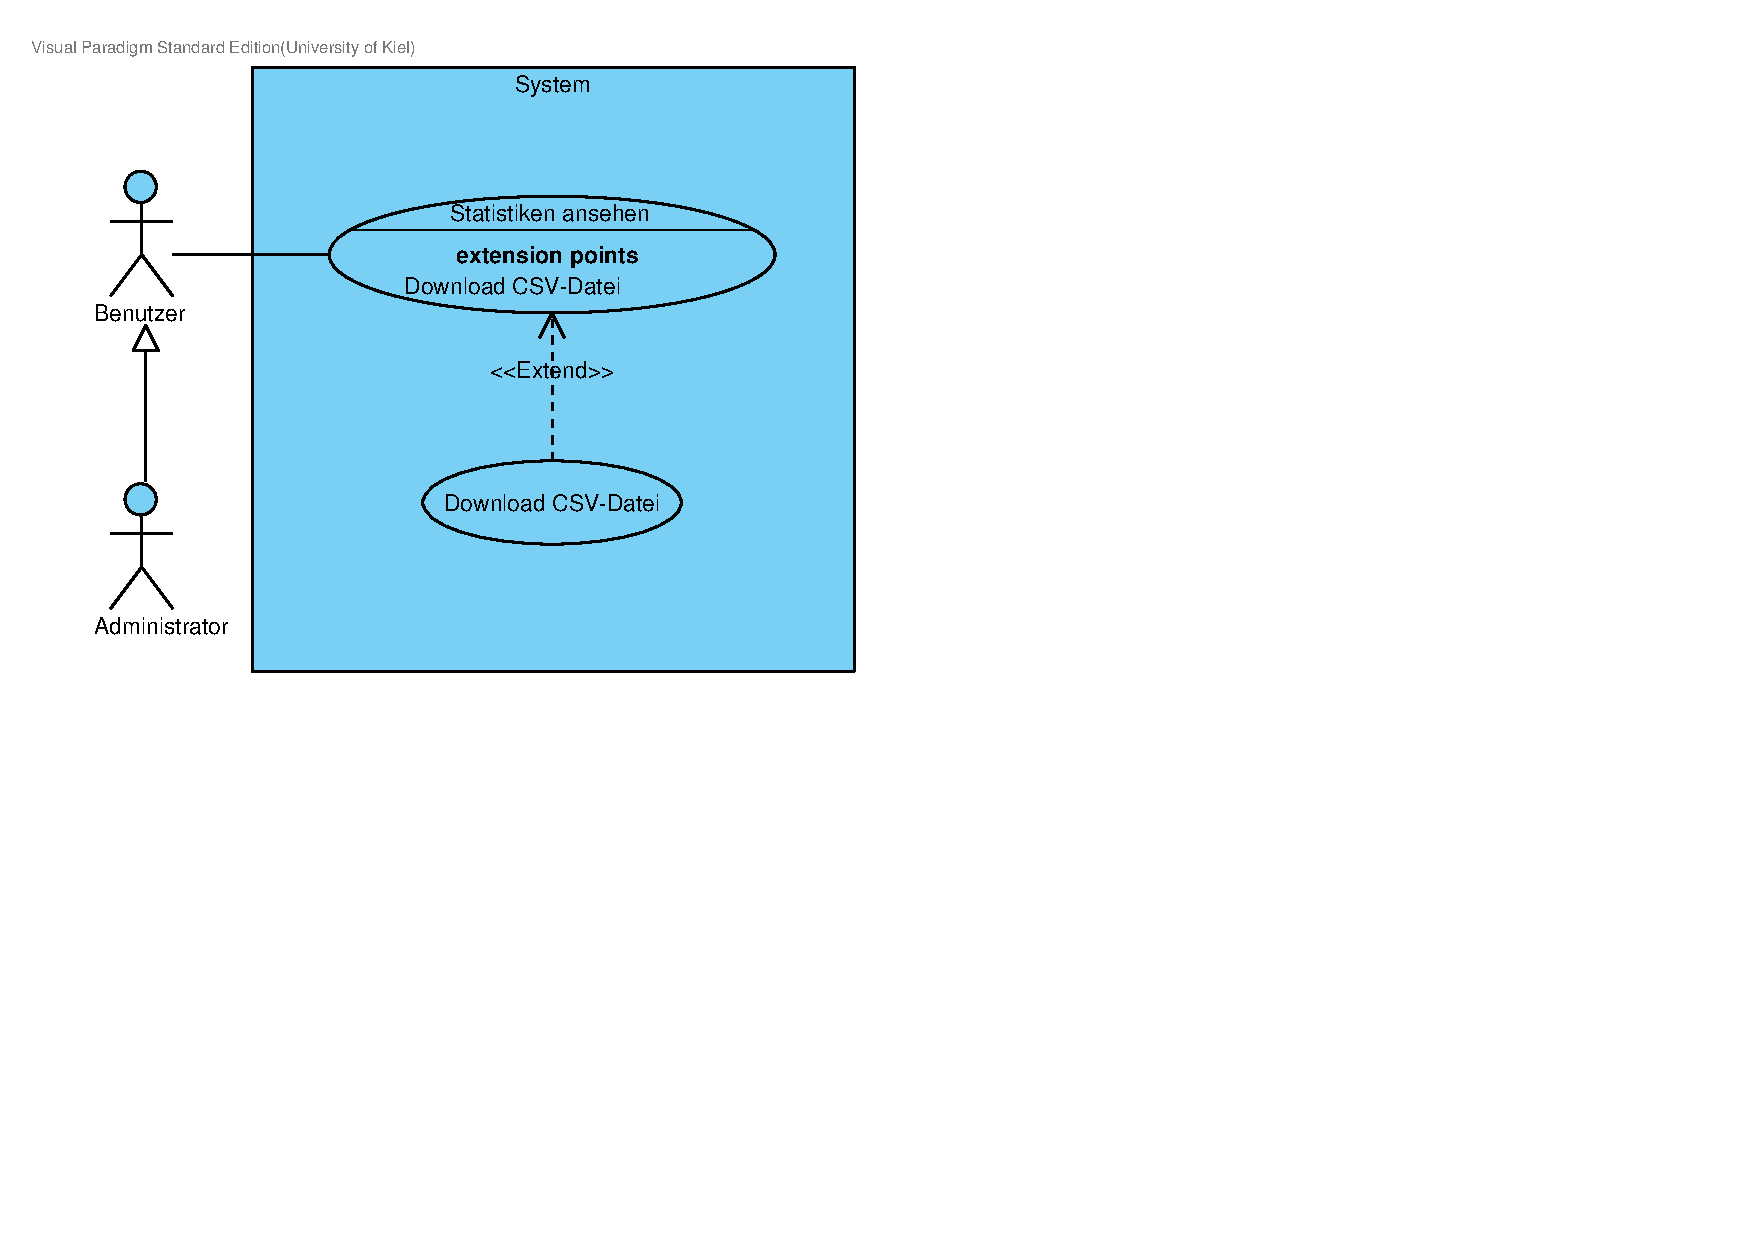
\includegraphics[width=\linewidth]{gfx/webseite/statistikfunktion.pdf}
          \caption{Use Case 1.6 Statistiken ansehen und als .csv-Datei exportieren}
	\end{figure}
        
\subsubsection{Statistiken ansehen}
	\begin{tabularx}{\textwidth}{|l|X|}
	\hline Use Case Nummer & 1.6.1\\ 
	\hline Use Case Name & Statistiken ansehen \\ 
	\hline Initiierender Akteur & Benutzer \\
	\hline Weitere Akteure &  \\
	\hline Kurzbeschreibung & Benutzer können grafische Statistiken einsehen \\
	\hline Vorbedingung & Der Benutzer ist eingeloggt. \\
	\hline Nachbedingung &   \\
	\hline \multicolumn{2}{|c|}{Funktionalität des Use Cases}\\
	\hline Ablauf & \begin{itemize}
		\item Der Benutzer wählt ``Statistiken anzeigen''.
		\item Eine Seite mit folgenden Statistiken wird angezeigt:
                      \begin{itemize}
                      \item Besucherzahl
                      \item summierte, gesammelte Punkte
                      \item summierte, erledigte Aktivitäten
                      \item beliebteste Aktivitäten
                      \end{itemize}
		\end{itemize} \\
	\hline Alternativen &  \\
	\hline Ausnahmen & \\
	\hline Benutzte Use Cases & \\
	\hline \multicolumn{2}{|c|}{Weitere Informationen} \\
	\hline Spezielle Anforderungen &  \\
	\hline Annahmen &  \\
	\hline
	\end{tabularx}

\subsubsection{Download CSV-Datei}
	\begin{tabularx}{\textwidth}{|l|X|}
	\hline Use Case Nummer & 1.6.2 \\ 
	\hline Use Case Name & Download CSV-Datei \\ 
	\hline Initiierender Akteur & Benutzer \\
	\hline Weitere Akteure &  \\
	\hline Kurzbeschreibung & Benutzer können die Rohdaten der Statistiken als .csv Datei exportieren und auf dem eigenen PC speichern. \\
	\hline Vorbedingung & Benutzer ist eingeloggt \\
	\hline Nachbedingung &  \\
	\hline \multicolumn{2}{|c|}{Funktionalität des Use Cases}\\
	\hline Ablauf & \begin{itemize}
                \item Der Benutzer klickt auf einen Download-Link bei einer der angezeigten, grafischen Statistiken.
                \item Es wird eine .csv-Datei generiert und dem Benutzer zum Download angeboten.
                \end{itemize}\\
	\hline Alternativen &  \\
	\hline Ausnahmen &  \\
	\hline Benutzte Use Cases &  \\
	\hline \multicolumn{2}{|c|}{Weitere Informationen} \\
	\hline Spezielle Anforderungen &  \\
	\hline Annahmen & \\
	\hline
	\end{tabularx}
        
%-----------------------------
\subsection{AdminBereich}
%-----------------------------
\subsection{Profilseite}

	\begin{figure}[H]
		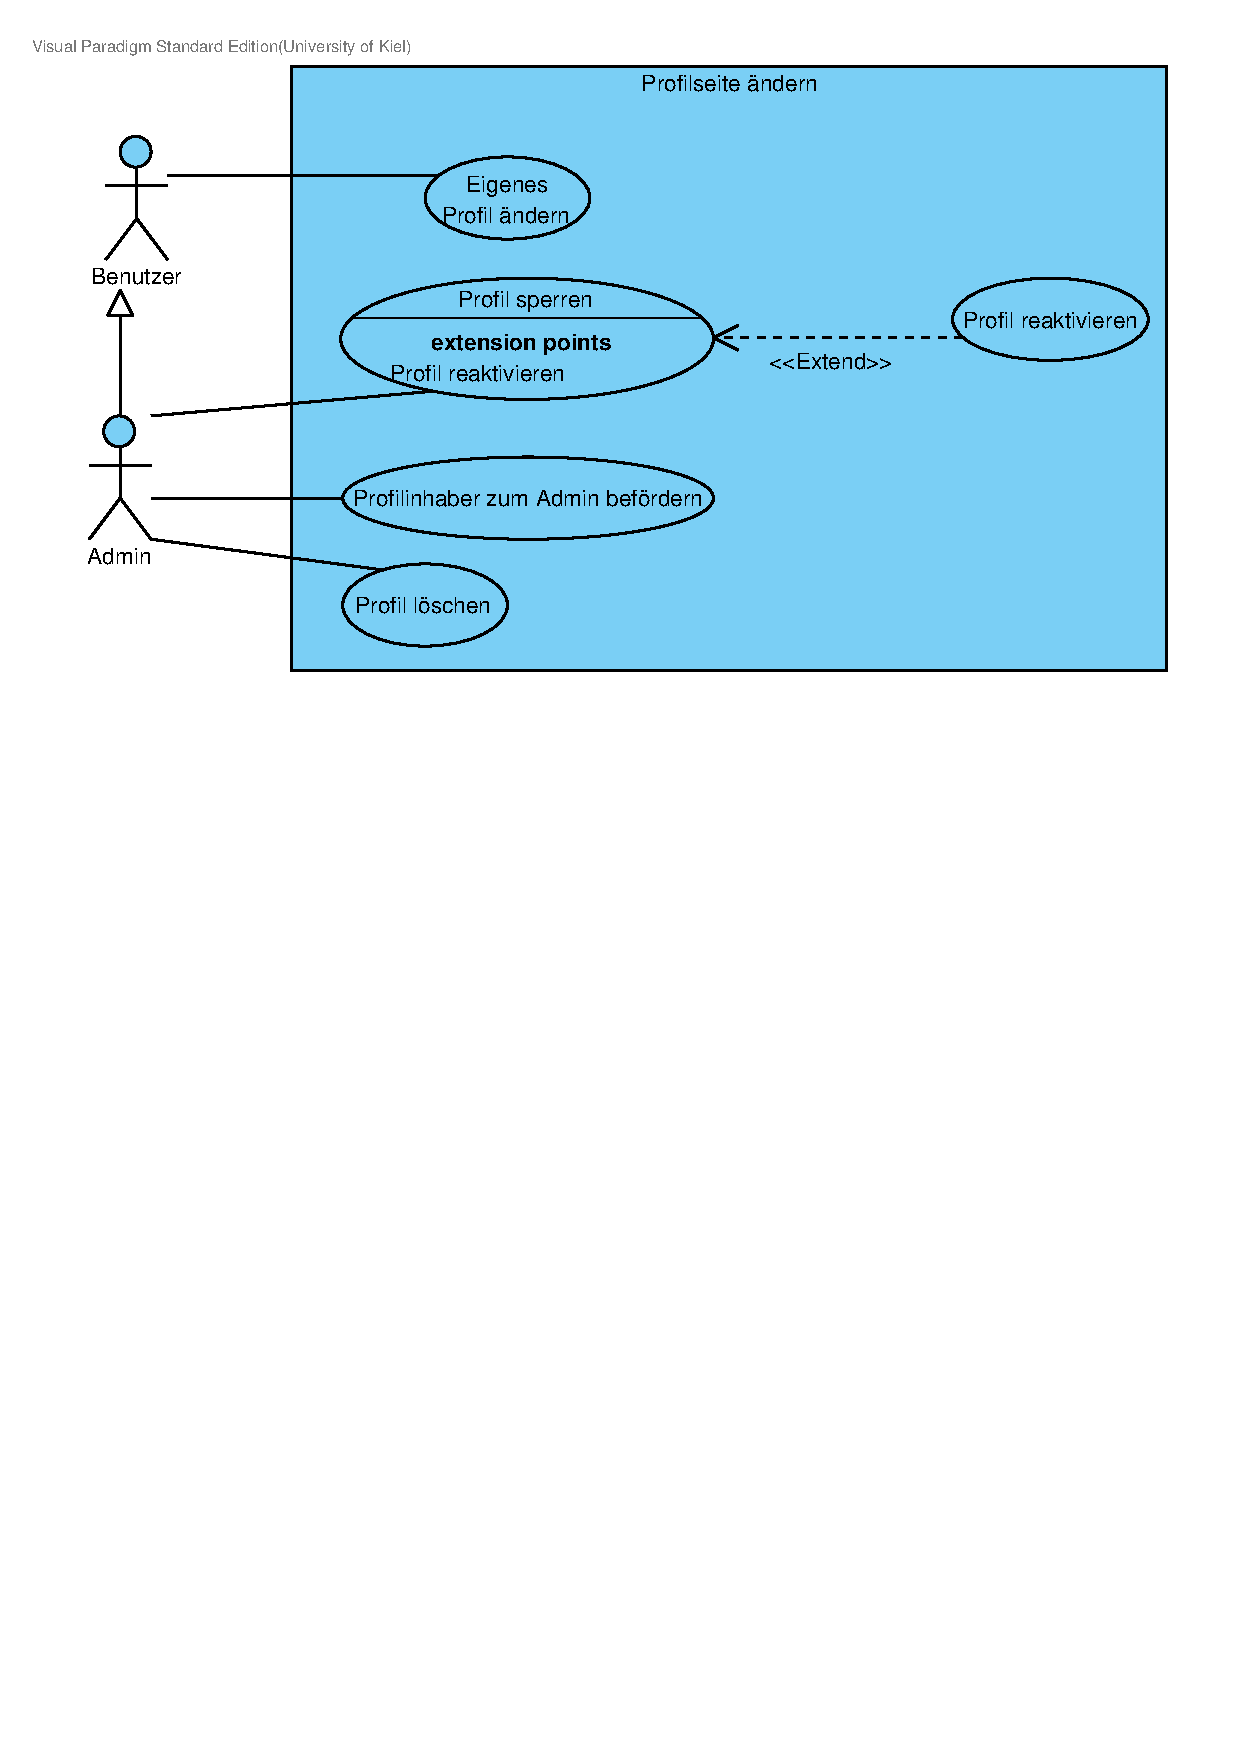
\includegraphics[width=\linewidth]{gfx/webseite/Profilseite.pdf}
		\caption{Use Case 1.8 Profilseite}
	\end{figure}
	\subsubsection{Profilseite \"andern}
		\begin{tabularx}{\textwidth}{|l|X|}
		\hline Use Case Nummer & 1.8 \\ 
		\hline Use Case Name & Profilseite \"andern \\ 
		\hline Initiierender Akteur & Benutzer \\
		\hline Weitere Akteure & \\
		\hline Kurzbeschreibung & Der Benutzer kann verschiedene Informationen seines Profils bearbeiten, wie Profilbild, Passwort, Benachrichtigungseinstellungen oder Fakultät und besitzt die Möglichkeit sein Profil zu löschen \\
		\hline Vorbedingung & Die Profilseite ist im Browser aufgerufen \\
		\hline Nachbedingung & Die Profilseite wird mit den vorgenommenen \"Anderungen angezeigt oder ist gel\"oscht worden \\
		\hline \multicolumn{2}{|c|}{Funktionalität des Use Cases}\\
		\hline Ablauf & \begin{itemize}
					\item Der Benutzer w\"ahlt eine Information, die er bearbeiten m\"ochte aus und bearbeitet diese
					\item Der Benutzer speichert die ge\"anderten Informationen und diese werden ins System \"ubernommen
				\end{itemize}\\
		\hline Alternativen & \\
		\hline Ausnahmen & \\
		\hline Benutzte Use Cases & \\
		\hline \multicolumn{2}{|c|}{Weitere Informationen} \\
		\hline Spezielle Anforderungen &  \\
		\hline Annahmen &  \\
		\hline
		\end{tabularx}
		
			\subsubsection{Profil sperren}
		\begin{tabularx}{\textwidth}{|l|X|}
		\hline Use Case Nummer & 1.8.1 \\ 
		\hline Use Case Name & Profil sperren \\ 
		\hline Initiierender Akteur & Admin \\
		\hline Weitere Akteure & - \\
		\hline Kurzbeschreibung & Der Admin kann ein Profil sperren, wenn irgendeine Form von Missverhalten vorliegt \\
		\hline Vorbedingung & Die Profilseite ist im Browser aufgerufen \\
		\hline Nachbedingung & Die Profilseite wird dem Admin als gesperrt angezeigt \\
		\hline \multicolumn{2}{|c|}{Funktionalität des Use Cases}\\
		\hline Ablauf & \begin{itemize}
					\item Der Admin \"offnet die Profilseite des zu sperrenden Profils
					\item Der Admin sperrt das entsprechende Profil, welches im Anschluss f\"ur Benutzer nicht mehr sichtbar und verwendbar ist
				\end{itemize}\\
		\hline Alternativen & - \\
		\hline Ausnahmen & - \\
		\hline Benutzte Use Cases & - \\
		\hline \multicolumn{2}{|c|}{Weitere Informationen} \\
		\hline Spezielle Anforderungen &  \\
		\hline Annahmen &  \\
		\hline
		\end{tabularx}
		
			\subsubsection{Profil reaktivieren}
		\begin{tabularx}{\textwidth}{|l|X|}
		\hline Use Case Nummer & 1.8.1.1 \\ 
		\hline Use Case Name & Profil reaktivieren \\ 
		\hline Initiierender Akteur & Admin \\
		\hline Weitere Akteure & - \\
		\hline Kurzbeschreibung & Admin kann ein zuvor gesperrtes Profil reaktivieren \\
		\hline Vorbedingung & Die gesperrte Profilseite ist im Browser aufgerufen \\
		\hline Nachbedingung & Die Profilseite ist wieder sichtbar \\
		\hline \multicolumn{2}{|c|}{Funktionalität des Use Cases}\\
		\hline Ablauf & \begin{itemize}
					\item Der Admin ruft ein gesperrtes Profil auf
					\item Der Admin reaktiviert das Profil, sodass es f\"ur alle Benutzer wieder sichtbar ist und der Profilinhaber wieder alle Funktionen nutzen kann
				\end{itemize}\\
		\hline Alternativen & - \\
		\hline Ausnahmen & - \\
		\hline Benutzte Use Cases & - \\
		\hline \multicolumn{2}{|c|}{Weitere Informationen} \\
		\hline Spezielle Anforderungen &  \\
		\hline Annahmen &  \\
		\hline
		\end{tabularx}
		
			\subsubsection{Profilinhaber zum Admin bef\"ordern}
		\begin{tabularx}{\textwidth}{|l|X|}
		\hline Use Case Nummer & 1.8.2 \\ 
		\hline Use Case Name & Profilinhaber zum Admin bef\"ordern \\ 
		\hline Initiierender Akteur & Admin \\
		\hline Weitere Akteure & Benutzer, der zum Admin wird \\
		\hline Kurzbeschreibung & Ein Admin kann einen Benutzer zum Admin ernennen und ihm so Administratorzugriff gew\"ahren \\
		\hline Vorbedingung & Die Profilseite ist im Browser aufgerufen \\
		\hline Nachbedingung & Die Profilseite wird im Browser angezeigt und der Benutzer ist im System als Admin registriert \\
		\hline \multicolumn{2}{|c|}{Funktionalität des Use Cases}\\
		\hline  Ablauf & \begin{itemize}
					\item Der Admin w\"ahlt das Profil des Benutzers aus, den er zum Admin bef\"ordern m\"ochte
					\item Der Admin bef\"ordert den Benutzer \"uber einen Men\"upunkt zum Administrator
				\end{itemize}\\
		\hline Alternativen & - \\
		\hline Ausnahmen & - \\
		\hline Benutzte Use Cases & - \\
		\hline \multicolumn{2}{|c|}{Weitere Informationen} \\
		\hline Spezielle Anforderungen &  \\
		\hline Annahmen & Das Profil des zu bef\"ordernden Benutzers ist nicht gesperrt \\
		\hline
		\end{tabularx}
		
			\subsubsection{Profil l\"oschen}
		\begin{tabularx}{\textwidth}{|l|X|}
		\hline Use Case Nummer & 1.8.3 \\ 
		\hline Use Case Name & Profil l\"oschen \\ 
		\hline Initiierender Akteur & Admin \\
		\hline Weitere Akteure & - \\
		\hline Kurzbeschreibung & Der Admin kann ausgew\"ahlte Profile l\"oschen \\
		\hline Vorbedingung & Die Profilseite ist im Browser aufgerufen \\
		\hline Nachbedingung & Das Profil ist aus dem System gel\"oscht \\
		\hline \multicolumn{2}{|c|}{Funktionalität des Use Cases}\\
		\hline  Ablauf & \begin{itemize}
					\item Der Admin w\"ahlt das zu löschende Profil aus
					\item Der Admin l\"oscht das Profil
				\end{itemize}\\
		\hline Alternativen & - \\
		\hline Ausnahmen & - \\
		\hline Benutzte Use Cases & - \\
		\hline \multicolumn{2}{|c|}{Weitere Informationen} \\
		\hline Spezielle Anforderungen & - \\
		\hline Annahmen & - \\
		\hline
		\end{tabularx}

%-----------------------------
\subsection{Android App}
	\begin{figure}[H]
	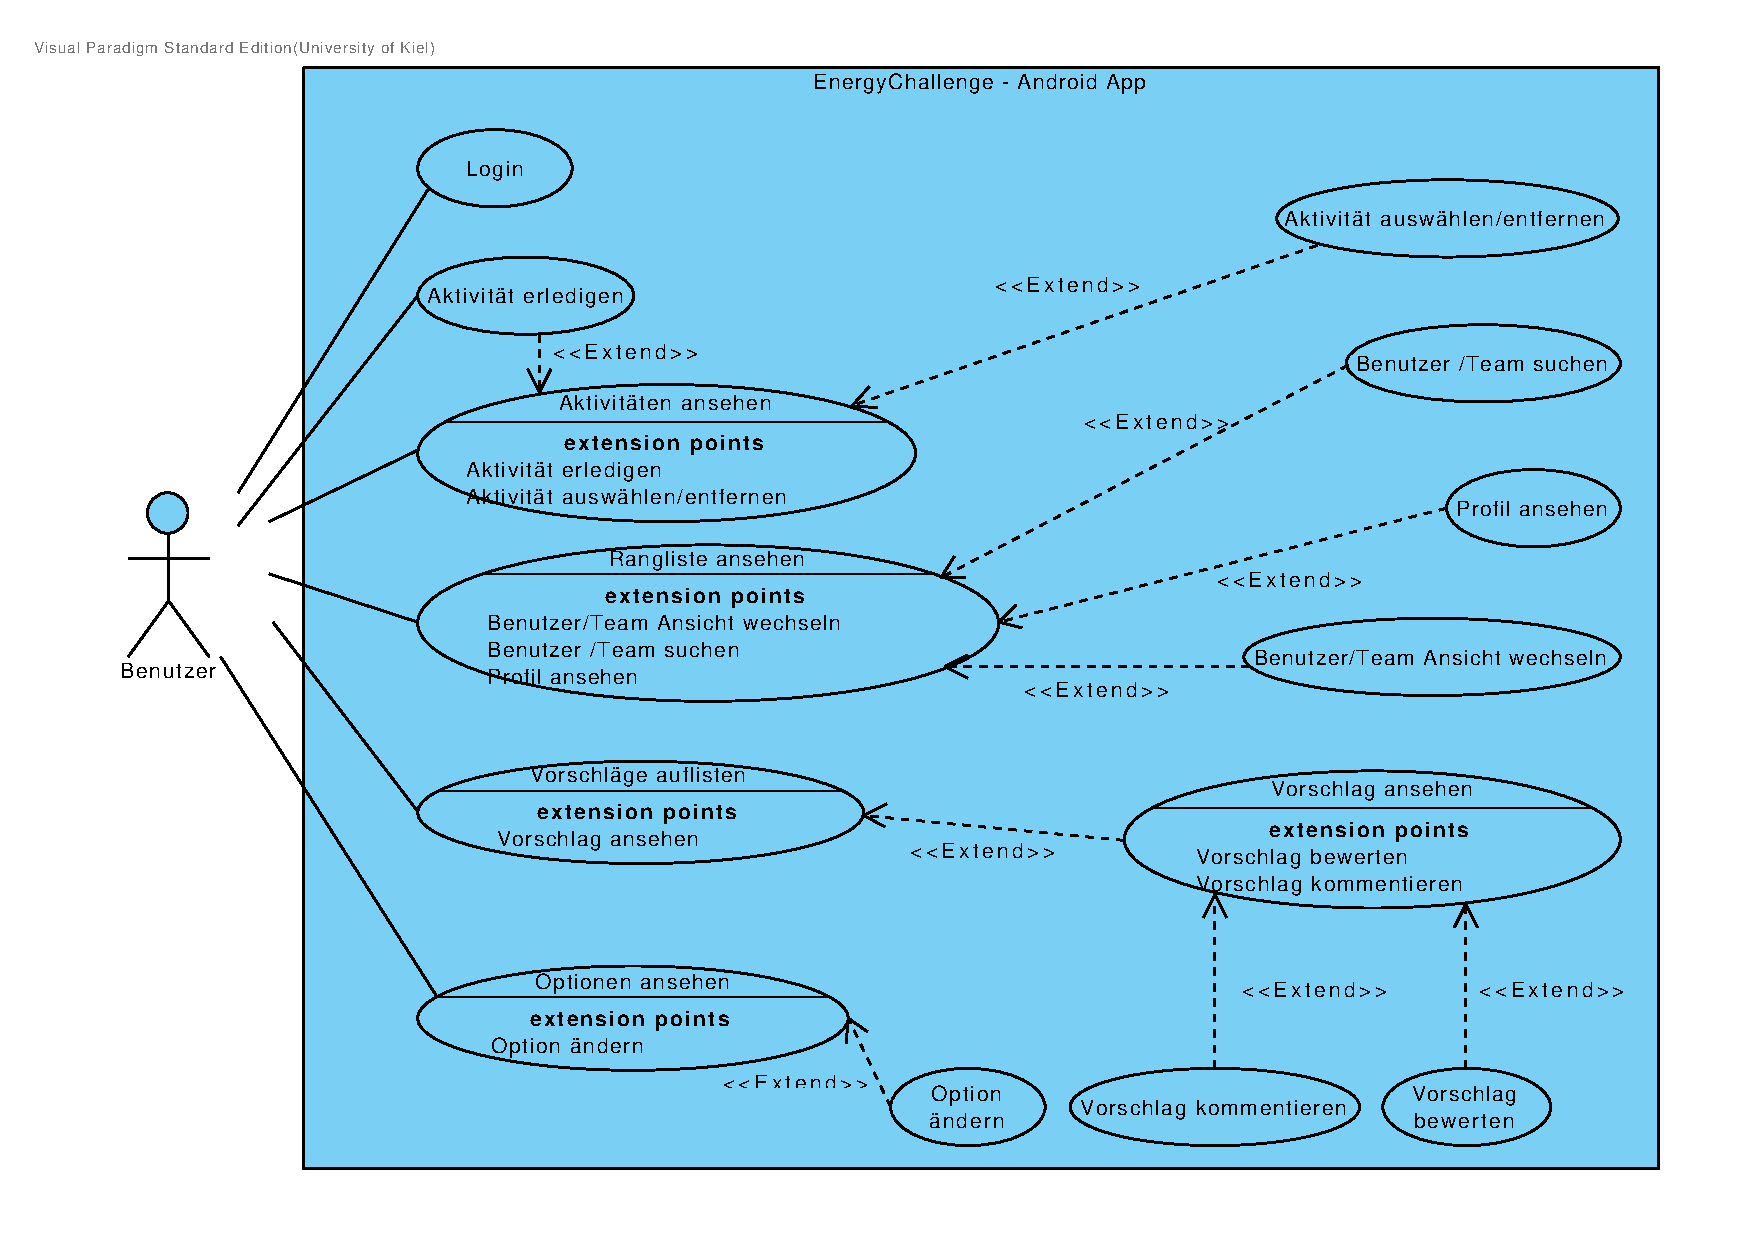
\includegraphics[width=\linewidth]{gfx/androidapp/overview.pdf}
	\caption{Use Case 2.1 Android App}
	\end{figure}

\subsubsection{Login}
	\begin{tabularx}{\textwidth}{|l|X|}
	\hline Use Case Nummer & 2.1 \\ 
	\hline Use Case Name & Login \\ 
	\hline Initiierender Akteur & Benutzer \\
	\hline Weitere Akteure &  \\
	\hline Kurzbeschreibung & Der Benutzer muss sich einmalig anmelden um die App nutzen zu können. \\
	\hline Vorbedingung & Benutzer hat sich noch nie in der App angemeldet. \\
	\hline Nachbedingung & Der Benutzer hat Zugriff auf die Funktionen der App. \\
	\hline \multicolumn{2}{|c|}{Funktionalität des Use Cases}\\
	\hline Ablauf & \begin{itemize}
		\item Der Benutzer startet die App und muss zunächst E-Mail-Adresse und Passwort eingeben.
		\item Der Benutzer drückt auf ``einloggen''.
	\end{itemize} \\
	\hline Alternativen &  \\
	\hline Ausnahmen & Bei falschen Login-Daten wird auf die Webseite verwiesen. \\
	\hline Benutzte Use Cases &  \\
	\hline \multicolumn{2}{|c|}{Weitere Informationen} \\
	\hline Spezielle Anforderungen &  \\
	\hline Annahmen & Der Benutzer hat sich auf der Webseite registriert. \\
	\hline
	\end{tabularx}

\subsubsection{Aktivit\"at erledigen}
	\begin{tabularx}{\textwidth}{|l|X|}
	\hline Use Case Nummer & 2.2 \\ 
	\hline Use Case Name & Aktivit\"at erledigen \\ 
	\hline Initiierender Akteur & Benutzer \\
	\hline Weitere Akteure &  \\
	\hline Kurzbeschreibung & Der Benutzer kann vom Startbildschirm der App aus favorisierte Aktivit\"aten erledigen. \\
	\hline Vorbedingung & Der Benutzer ist eingeloggt. \\
	\hline Nachbedingung & Die gewählte Aktivit\"at wurde als erledigt markiert \\
	\hline \multicolumn{2}{|c|}{Funktionalität des Use Cases}\\
	\hline Ablauf & \begin{itemize}
		\item Benutzer drückt auf eine Aktivit\"at.
		\item Benutzer best\"atigt, dass er die Aktivit\"at als erledigt markieren möchte.
	\end{itemize} \\
	\hline Alternativen &  \\
	\hline Ausnahmen &  \\
	\hline Benutzte Use Cases &  \\
	\hline \multicolumn{2}{|c|}{Weitere Informationen} \\
	\hline Spezielle Anforderungen &  \\
	\hline Annahmen &  \\
	\hline
	\end{tabularx}

\subsubsection{Aktivit\"aten ansehen}
	\begin{tabularx}{\textwidth}{|l|X|}
	\hline Use Case Nummer & 2.3 \\ 
	\hline Use Case Name & Aktivi\"aten ansehen \\ 
	\hline Initiierender Akteur & Benutzer \\
	\hline Weitere Akteure &  \\
	\hline Kurzbeschreibung & Der Benutzer kann eine Liste mit den von verf\"ugbaren Aktivit\"aten ansehen. \\
	\hline Vorbedingung & Der Benutzer ist eingeloggt. \\
	\hline Nachbedingung & Eine Liste mit allen Aktitvitäten wird angezeigt. \\
	\hline \multicolumn{2}{|c|}{Funktionalität des Use Cases}\\
	\hline Ablauf & \begin{itemize}
		\item Der Benutzer drückt im Menü auf "Aktivit\"aten.
		\item Eine Übersicht über alle vom Benutzer gewählten Aktivit\"aten wird angezeigt.
	\end{itemize} \\
	\hline Alternativen &  \\
	\hline Ausnahmen &  \\
	\hline Benutzte Use Cases &  \\
	\hline \multicolumn{2}{|c|}{Weitere Informationen} \\
	\hline Spezielle Anforderungen &  \\
	\hline Annahmen &  \\
	\hline
	\end{tabularx}

\subsubsection{Rangliste ansehen}
	\begin{tabularx}{\textwidth}{|l|X|}
	\hline Use Case Nummer & 2.4 \\ 
	\hline Use Case Name & Rangliste ansehen\\ 
	\hline Initiierender Akteur & Benutzer \\
	\hline Weitere Akteure &  \\
	\hline Kurzbeschreibung & Der Benutzer kann die aktuelle Rangliste der Benutzer und Teams ansehen. \\
	\hline Vorbedingung & Der Benutzer ist eingeloggt. \\
	\hline Nachbedingung & Die Rangliste wird angezeigt. \\
	\hline \multicolumn{2}{|c|}{Funktionalität des Use Cases}\\
	\hline Ablauf & \begin{itemize}
		\item Der Benutzer drückt im Menü auf "Rangliste".
		\item Die Rangliste wird angezeigt.
	\end{itemize} \\
	\hline Alternativen &  \\
	\hline Ausnahmen &  \\
	\hline Benutzte Use Cases &  \\
	\hline \multicolumn{2}{|c|}{Weitere Informationen} \\
	\hline Spezielle Anforderungen &  \\
	\hline Annahmen &  \\
	\hline
	\end{tabularx}

\subsubsection{Benutzer/Team Ansicht ändern}
	\begin{tabularx}{\textwidth}{|l|X|}
	\hline Use Case Nummer & 2.4.1 \\ 
	\hline Use Case Name & Benutzer/Team Ansicht \"andern \\ 
	\hline Initiierender Akteur & Benutzer \\
	\hline Weitere Akteure &  \\
	\hline Kurzbeschreibung & Der Benutzer kann zwischen der Benutzer- und der Team-Rangliste wechseln \\
	\hline Vorbedingung & Der Benutzer ist in der Ranglisten Ansicht. \\
	\hline Nachbedingung & Die Benutzer oder Team Rangliste wird angezeigt. \\
	\hline \multicolumn{2}{|c|}{Funktionalität des Use Cases}\\
	\hline Ablauf & \begin{itemize}
		\item Der Benutzer wischt in der Team-Rangliste nach rechts über den Bildschirm.
		\item Die Benutzer-Rangliste wird angezeigt.
	\end{itemize} \\
	\hline Alternativen & \begin{itemize}
		\item Der Benutzer wischt in der Benutzer-Rangliste nach links über den Bildschirm.
		\item Die Team-Rangliste wird angezeigt.
                \end{itemize} \\
	\hline Ausnahmen &  \\
	\hline Benutzte Use Cases &  \\
	\hline \multicolumn{2}{|c|}{Weitere Informationen} \\
	\hline Spezielle Anforderungen &  \\
	\hline Annahmen &  \\
	\hline
	\end{tabularx}

\subsubsection{Profil ansehen}
	\begin{tabularx}{\textwidth}{|l|X|}
	\hline Use Case Nummer & 2.4.2 \\ 
	\hline Use Case Name & Profil ansehen \\ 
	\hline Initiierender Akteur & Benutzer \\
	\hline Weitere Akteure &  \\
	\hline Kurzbeschreibung & Der Benutzer kann die Profile von anderen Benutzern und Teams ansehen \\
	\hline Vorbedingung & Der Benutzer ist eingeloggt und befindet sich in der Ranglistenansicht. \\
	\hline Nachbedingung & Das ausgewählte Profil wird angezeigt. \\
	\hline \multicolumn{2}{|c|}{Funktionalität des Use Cases}\\
	\hline Ablauf & \begin{itemize}
		\item Der Benutzer drückt auf einen Benutzer oder ein Team.
		\item Das Profil des entsprechenden Benutzers oder Teams wird angezeigt.
	\end{itemize} \\
	\hline Alternativen &  \\
	\hline Ausnahmen &  \\
	\hline Benutzte Use Cases &  \\
	\hline \multicolumn{2}{|c|}{Weitere Informationen} \\
	\hline Spezielle Anforderungen &  \\
	\hline Annahmen &  \\
	\hline
	\end{tabularx}

\subsubsection{Benutzer/Team suchen}
	\begin{tabularx}{\textwidth}{|l|X|}
	\hline Use Case Nummer & 2.4.3 \\ 
	\hline Use Case Name & Suche \\ 
	\hline Initiierender Akteur & Benutzer \\
	\hline Weitere Akteure &  \\
	\hline Kurzbeschreibung & Benutzer kann nach anderen Benutzern und Teams suchen. \\
	\hline Vorbedingung & Benutzer ist eingeloggt. \\
	\hline Nachbedingung & Die Suchergebnisse werden angezeigt. \\
	\hline \multicolumn{2}{|c|}{Funktionalität des Use Cases}\\
	\hline Ablauf & \begin{itemize}
		\item Der Benutzer drückt auf das Suchsymbol auf der Hauptseite der App.
                \item Eine Suchzeile zur Eingabe von Suchbegriffen öffnet sich.
                \item Der Benutzer gibt einen Suchbegriff ein.
		\item Der Benutzer drückt auf ``Suchen''.
		\item Die Suchergebnisse werden angezeigt.
	\end{itemize} \\
	\hline Alternativen & \\
	\hline Ausnahmen & Wenn keine Benutzer oder Teams mit dem gesuchten Namen gefunden werden, wird ``Ihre Suche lieferte keine Ergebnisse'' angezeigt. \\
	\hline Benutzte Use Cases &  \\
	\hline \multicolumn{2}{|c|}{Weitere Informationen} \\
	\hline Spezielle Anforderungen &  \\
	\hline Annahmen &  \\
	\hline
	\end{tabularx}

\subsubsection{Vorschl\"age auflisten}
	\begin{tabularx}{\textwidth}{|l|X|}
	\hline Use Case Nummer & 2.5 \\ 
	\hline Use Case Name & Vorschl\"age auflisten \\ 
	\hline Initiierender Akteur & Benutzer \\
	\hline Weitere Akteure &  \\
	\hline Kurzbeschreibung & Alle bislang abgegebenen Vorschl\"age werden dem Benutzer angezeigt. \\
	\hline Vorbedingung & Der Benutzer ist eingeloggt. \\
	\hline Nachbedingung & Die Vorschl\"age werden angezeigt. \\
	\hline \multicolumn{2}{|c|}{Funktionalität des Use Cases}\\
	\hline Ablauf & \begin{itemize}
		\item Der Benutzer drückt im Men\"u auf der Hauptseite der App auf "Vorschl\"age".
		\item Eine Liste mit allen bislang abgegebenen Vorschlägen wird angezeigt.
	\end{itemize} \\
	\hline Alternativen &  \\
	\hline Ausnahmen &  \\
	\hline Benutzte Use Cases &  \\
	\hline \multicolumn{2}{|c|}{Weitere Informationen} \\
	\hline Spezielle Anforderungen &  \\
	\hline Annahmen &  \\
	\hline
	\end{tabularx}

\subsubsection{Vorschlag ansehen}
	\begin{tabularx}{\textwidth}{|l|X|}
	\hline Use Case Nummer & 2.5.1 \\ 
	\hline Use Case Name & Vorschlag ansehen \\ 
	\hline Initiierender Akteur & Benutzer \\
	\hline Weitere Akteure &  \\
	\hline Kurzbeschreibung & Der Benutzer kann sich einzelne Vorschl\"age ansehen, ihm werden dabei die Kommentare und Bewertungen zu dem Vorschlage angezeigt. \\
	\hline Vorbedingung & Benutzer ist eingeloggt und befindet sich in der Vorschlagsansicht. \\
	\hline Nachbedingung & Der ausgewählte Vorschlag und alle zugehörigen Kommentare sowie die durchschnittliche Bewertung des Vorschlages werden angezeigt. \\
	\hline \multicolumn{2}{|c|}{Funktionalität des Use Cases}\\
	\hline Ablauf & \begin{itemize}
		\item Der Benutzer drückt in der Liste der Vorschläge auf einen Vorschlag.
		\item Dem Benutzer wird die Beschreibung des Vorschlags und alle zugehörigen Kommentare, sowie eine durchschnittliche Bewertung angezeigt.
	\end{itemize} \\
	\hline Alternativen &  \\
	\hline Ausnahmen & \begin{itemize}
        	\item Wenn zu einem Vorschlag kein Kommentar existiert, wird angezeigt, dass bislang keine Kommentare zu dem Vorschlag exisiteren.
                \item Wenn zu einem Vorschlag keine Bewertung existiert, wird angezeigt, dass bislang keine Bewertungen zu dem Vorschlag existieren. 
                \end{itemize} \\
	\hline Benutzte Use Cases &  \\
	\hline \multicolumn{2}{|c|}{Weitere Informationen} \\
	\hline Spezielle Anforderungen &  \\
	\hline Annahmen &  \\
	\hline
	\end{tabularx}

\subsubsection{Vorschlag bewerten}
	\begin{tabularx}{\textwidth}{|l|X|}
	\hline Use Case Nummer & 2.5.1.1 \\ 
	\hline Use Case Name & Vorschlag bewerten \\ 
	\hline Initiierender Akteur & Benutzer \\
	\hline Weitere Akteure &  \\
	\hline Kurzbeschreibung & Der Benutzer kann Vorschl\"age mit 1 bis 5 Sternen bewerten. \\
	\hline Vorbedingung & \begin{itemize}
        	\item Der Benutzer ist eingeloggt.
                \item Der Benutzer befindet sich in Ansicht des Vorschlags.
                \item Der Benutzer hat den Vorschlag noch nicht bewertet.
                \end{itemize} \\
	\hline Nachbedingung & Der Benutzer hat den Vorschlag bewertet. \\
	\hline \multicolumn{2}{|c|}{Funktionalität des Use Cases}\\
	\hline Ablauf & \begin{itemize}
		\item Der Benutzer w\"ahlt die abzugebende Bewertung in der Ansicht des Vorschlags.
		\item Der Benutzer klickt auf ``Bewertung abgeben''.
	\end{itemize} \\
	\hline Alternativen &  \\
	\hline Ausnahmen &  \\
	\hline Benutzte Use Cases &  \\
	\hline \multicolumn{2}{|c|}{Weitere Informationen} \\
	\hline Spezielle Anforderungen &  \\
	\hline Annahmen &  \\
	\hline
	\end{tabularx}

\subsubsection{Vorschlag kommentieren}
	\begin{tabularx}{\textwidth}{|l|X|}
	\hline Use Case Nummer & 2.5.1.2 \\ 
	\hline Use Case Name & Vorschlag kommentieren \\ 
	\hline Initiierender Akteur & Benutzer \\
	\hline Weitere Akteure &  \\
	\hline Kurzbeschreibung & Der Benutzer kann einen Vorschlag kommenieren. \\
	\hline Vorbedingung & \begin{itemize}
        	\item Der Benutzer ist eingeloggt.
                \item Der Benutzer befindet sich in Ansicht des Vorschlags.
                \item Der Benutzer hat den Vorschlag noch nicht kommentiert.
                \end{itemize} \\
	\hline Nachbedingung & Der Benutzer hat den Vorschlag kommentiert. \\
	\hline \multicolumn{2}{|c|}{Funktionalität des Use Cases}\\
	\hline Ablauf & \begin{itemize}
		\item Der Benutzer drückt auf "Kommentieren".
                \item Ein Textfeld zur Eingabe des Kommentars erscheint.
		\item Der Benutzer schreibt einen Kommentar in das Textfeld.
		\item Der Benutzer drückt auf ``Kommentar abgeben''.
	\end{itemize} \\
	\hline Alternativen &  \\
	\hline Ausnahmen &  \\
	\hline Benutzte Use Cases &  \\
	\hline \multicolumn{2}{|c|}{Weitere Informationen} \\
	\hline Spezielle Anforderungen &  \\
	\hline Annahmen &  \\
	\hline
	\end{tabularx}

\subsubsection{Optionen anzeigen}
	\begin{tabularx}{\textwidth}{|l|X|}
	\hline Use Case Nummer & 2.6 \\ 
	\hline Use Case Name & Optionen \\ 
	\hline Initiierender Akteur & Benutzer \\
	\hline Weitere Akteure &  \\
	\hline Kurzbeschreibung & Der Benutzer kann die Einstellungen zum Verhalten von Benachrichtigungen einsehen. \\
	\hline Vorbedingung & Der Benutzer ist eingeloggt. \\
	\hline Nachbedingung & Die aktuell gültigen Einstellungen zum Verhalten der Benachrichtigungen werden angezeigt. \\
	\hline \multicolumn{2}{|c|}{Funktionalität des Use Cases}\\
	\hline Ablauf & \begin{itemize}
		\item Der Benutzer drückt im Menü der App auf "Optionen".
		\item Die aktuell gültigen Einstellungen zum Verhalten der Benachrichtigungen werden angezeigt.
	\end{itemize} \\
	\hline Alternativen &  \\
	\hline Ausnahmen &  \\
	\hline Benutzte Use Cases &  \\
	\hline \multicolumn{2}{|c|}{Weitere Informationen} \\
	\hline Spezielle Anforderungen &  \\
	\hline Annahmen &  \\
	\hline
	\end{tabularx}

\subsubsection{Option \"andern}
	\begin{tabularx}{\textwidth}{|l|X|}
	\hline Use Case Nummer & 2.6.1 \\ 
	\hline Use Case Name & Option \"andern \\ 
	\hline Initiierender Akteur & Benutzer \\
	\hline Weitere Akteure &  \\
	\hline Kurzbeschreibung & Der Benutzer kann das Verhalten der Benachrichtigungen verändern. \\
	\hline Vorbedingung & Der Benutzer ist eingeloggt und befindet sich in der Optionenansicht der App. \\
	\hline Nachbedingung & Die Einstellung der Benachrichtigung wurde entsprechend der Auswahl des Benutzer geändert. \\
	\hline \multicolumn{2}{|c|}{Funktionalität des Use Cases}\\
	\hline Ablauf & Der Benutzer aktiviert die Benachrichtigungen über ausgewählte, aber nicht erledigte Aktivitäten. \\
	\hline Alternativen & Der Benutzer deaktiviert die Benachrichtigungen über ausgewählte, aber nicht erledigte Aktivitäten. \\
	\hline Ausnahmen &  \\
	\hline Benutzte Use Cases &  \\
	\hline \multicolumn{2}{|c|}{Weitere Informationen} \\
	\hline Spezielle Anforderungen &  \\
	\hline Annahmen &  \\
	\hline
	\end{tabularx}

%%Tabellen Muster
%\subsubsection{title}
%	\begin{tabularx}{\textwidth}{|l|X|}
%	\hline Use Case Nummer &  \\ 
%	\hline Use Case Name &  \\ 
%	\hline Initiierender Akteur &  \\
%	\hline Weitere Akteure &  \\
%	\hline Kurzbeschreibung &  \\
%	\hline Vorbedingung &  \\
%	\hline Nachbedingung &  \\
%	\hline \multicolumn{2}{|c|}{Funktionalität des Use Cases}\\
%	\hline Ablauf &  \\
%	\hline Alternativen &  \\
%	\hline Ausnahmen &  \\
%	\hline Benutzte Use Cases &  \\
%	\hline \multicolumn{2}{|c|}{Weitere Informationen} \\
%	\hline Spezielle Anforderungen &  \\
%	\hline Annahmen &  \\
%	\hline
%	\end{tabularx}

%------------------------------------------------
% Produktdaten
%------------------------------------------------
\section{Produktdaten}
Die Daten werden in einer Datenbank gespeichert \\
\begin{itemize}
\item Benutzerdaten: 
\begin{itemize}
\item Vorname
\item Name
\item E-Mail Adresse
\item Passwort (verschlüsselt)
\item Foto
\item Institut
\item Rolle (Benutzer, Administrator)
\item Teamname
\item ausgewählte Aktivitäten
\item erledigte Aktivitäten
\item Punktzahl
\item laufende Challenges
\item abgeschlossene Challenges
\end{itemize}

\item Aktivitäten: 
\begin{itemize}
\item Aktivitätsname
\item Häufigkeitsattribut (täglich, wöchentlich, etc.)
\item Punkte für Aktivität
\item Challengenamen
\item Challengezeitraum
\item Challengepunkte
\end{itemize}

\item Vorschläge:
\begin{itemize}
\item Vorschlagsname
\item vorgeschlagene Punktzahl
\item Vorschlagserläuterung (wenn aus Name nicht ersichtlich)
\item Kommentare
\item Bewertungen
\end{itemize}

\item Statistik:
\begin{itemize}
\item Besucherzahl (Anzahl Logins)
\item Besucherzahl (Anzahl Startseitenzugriffe)
\end{itemize}
\end{itemize}







%------------------------------------------------
% Produktleistung
%------------------------------------------------
\section{Produktleistungen}

\subsection{L100/Client} 
Das System unterstützt die Anmeldung mehrerer Benutzer mit mehreren Clients (Webseite und/oder App) an einen zentralen Server. Der Client beinhaltet die Möglichkeit, Befehle vom Nutzer anzunehmen und sie an den Server weiterzuleiten. 

\subsection{L110/Antwortzeit} 
Nutzeranfragen werden in wenigen Sekunden bearbeitet, damit ein schnelle Nutzung ermöglicht wird. Im Falle, dass zwischen Client und Server Objekte, wie Fotos zum Upload, verschickt werden, kann die Antwortzeit minimal ansteigen. 

\subsection{L110/Ladezeit} 
Die Webseite benötigt nur eine kurze Zeit zum Starten. Diese ist natürlich von äußeren Faktoren (benutzter PC, Internetverbindung, etc.) abhängig. 

\subsection{L200/Server} 
Das System hat einen zentralen Server. Der Server bietet den Zugriff auf die Webseite und die die App an. 

\subsection{L300/Datenbank} 
Das System besitzt eine integrierte Datenbank. In der Datenbank werden alle relevanten Daten zum Betrieb der Webseite und der App gespeichert. Dies sind die Aktivitäten, Profile, Statistiken, Team-/Benutzerlisten, Ranglisten und Vorschläge, sowie Kommentare und Bewertungen.

\subsection{L310/Statistik} 
Die Datenbank erstellt Statistiken über die Besucherzahlen, die Anzahl aller erledigten Aktivitäten, die Anzahl aller gesammelten Punkte und die beliebtesten Aktivitäten. Des Weiteren wird mit der Datenbank eine Rangliste der Benutzer mit den meisten Punkten erstellt.

\subsection{L400/Benutzersicherheit} 
Die Webseiten- und die Appoberfläche sind so aufgebaut, dass der Benutzer keine unbeabsichtigten Eingaben tätigen kann, ohne, dass nachgefragt wird, ob er diese tätigen möchte. Nur ein Systemadministrator kann die Webseite und die App vom Server entfernen oder hinzufügen.


%------------------------------------------------
% Benutzeroberflache
%------------------------------------------------
\section{Benutzeroberfl\"ache}
\subsection{Webseite}
\subsubsection{Grundlegende Anforderungen}
Die Benutzeroberfläche der Website soll intuitiv aufgebaut und einfach bedienbar sein. Aus diesem Grund soll die Website gängigen Layoutkonventionen entsprechen und besteht deshalb aus einer Kopfzeile und einem linksspaltigen Navigationsmenü, die beide von jeder Stelle der Website aus erreichbar sein sollen. Die Website ist in erster Linie für die Bedienung mit der Maus ausgelegt, soll jedoch auch auf einem Touchscreen bedienbar sein.\\
Bevor der Benutzer sich angemeldet hat, wird ihm nur das Projekt präsentiert und man gibt ihm die Möglichkeit sich anzumelden oder für das Projekt zu registrieren. \\
Wenn der Benutzer angemeldet ist, kann er über das Menü zwischen den einzelnen Seiten navigieren. In der Kopfzeile werden ihm stets seine persönlichen Informationen eingeblendet (wie z.B. neue Benachrichtigungen) und es gibt hier die Möglichkeit sich wieder von der Website abzumelden.
\subsubsection{Navigationsstruktur}
\begin{figure}[H]
	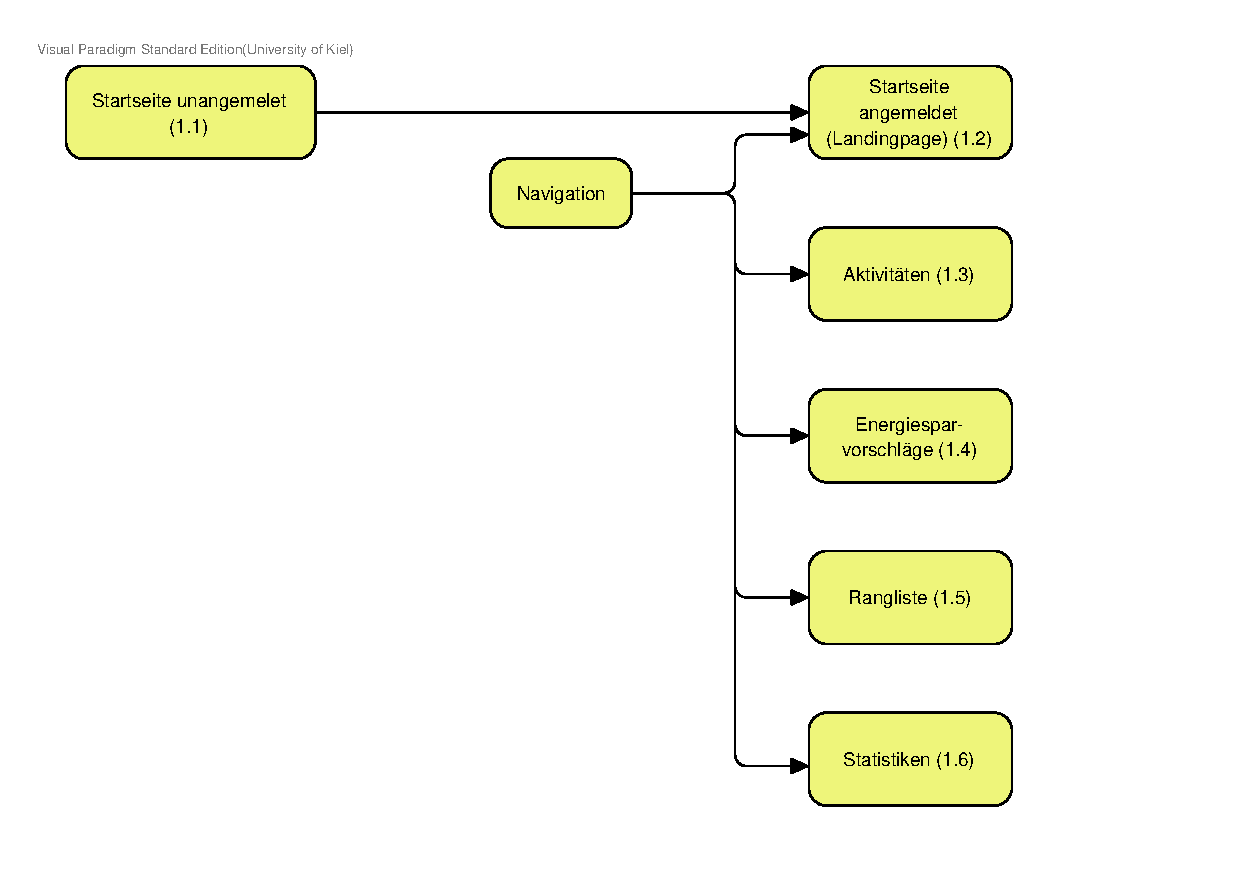
\includegraphics[width=\linewidth]{gfx/guinavigation/GUI-Navigation-Website.pdf}
\end{figure}
\subsubsection{GUI-Entwurfsvorschläge}
Die folgenden Grafiken stellen Entwurfsvorschläge für die Benutzeroberfläche dar. Die in gelb eingezeichneten Nummern sind die IDs der Use Cases, die an dieser Stelle verwendet werden.
\begin{figure}[H]
	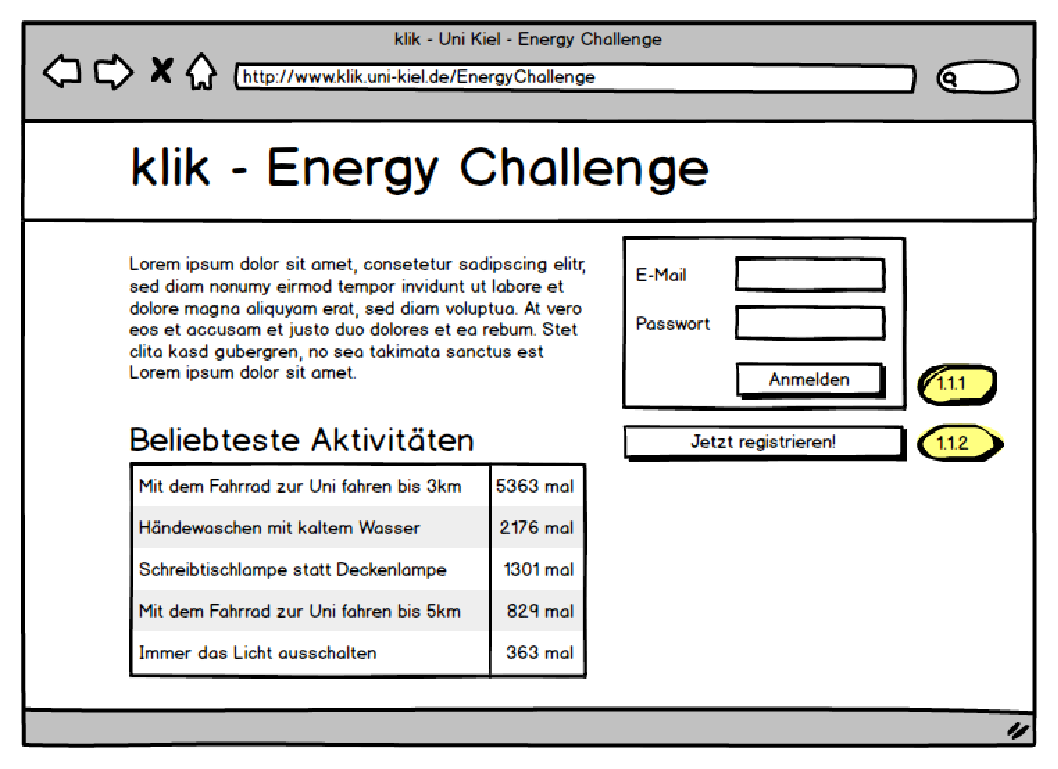
\includegraphics[width=\linewidth]{gfx/mockups/website-startseite.pdf}
	\caption{Startbildschirm für unangemeldete Benutzer}
\end{figure}
\begin{figure}[H]
	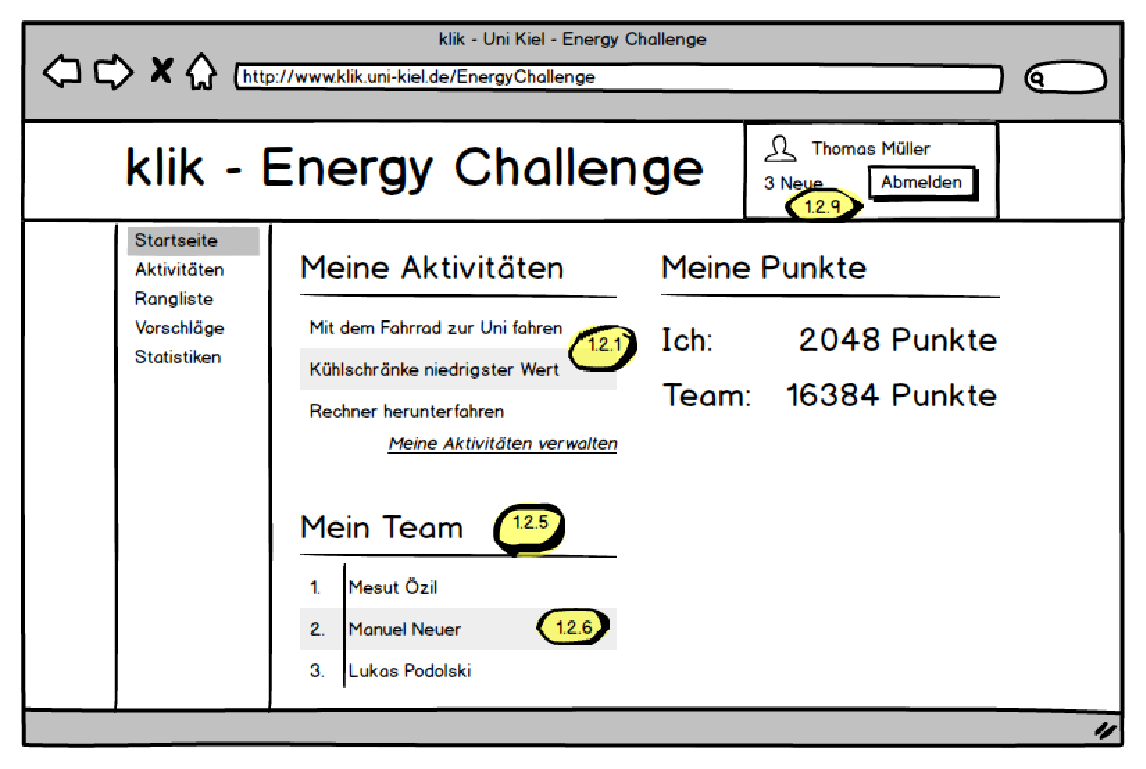
\includegraphics[width=\linewidth]{gfx/mockups/website-landingpage.pdf}
		\caption{Startbildschirm für angemeldete Benutzer}
\end{figure}
\begin{figure}[H]
	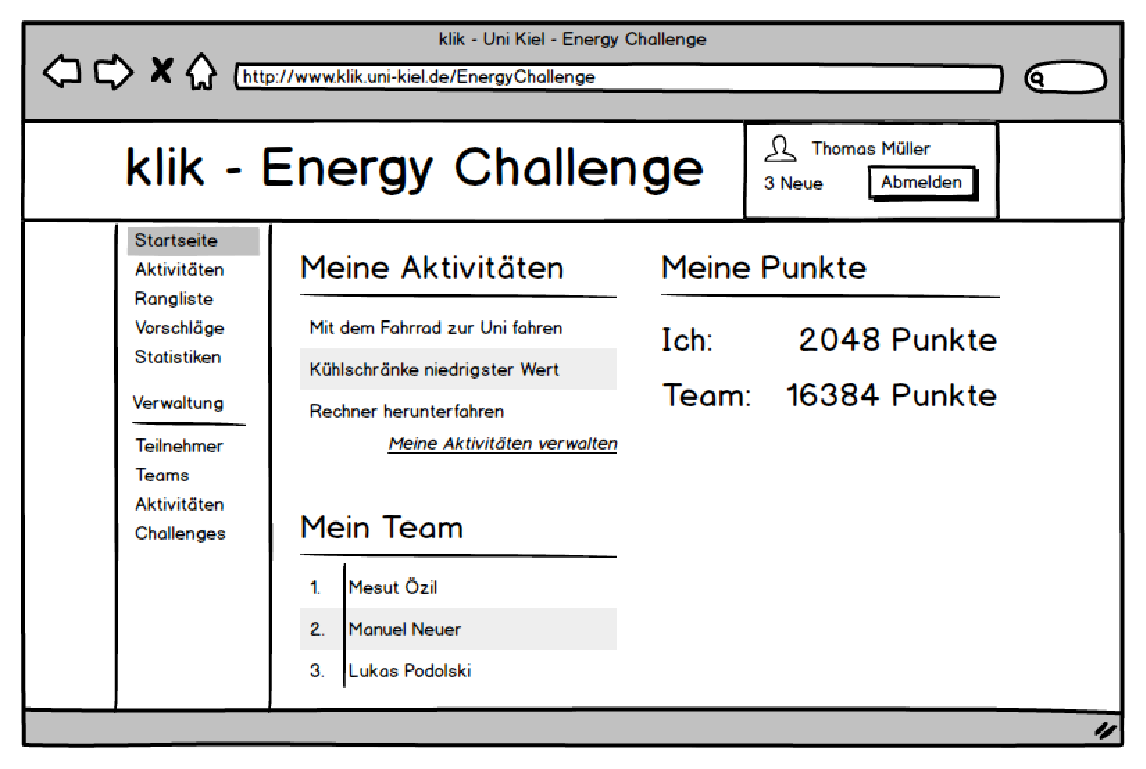
\includegraphics[width=\linewidth]{gfx/mockups/website-landingpage-admin.pdf}
			\caption{Startbildschirm für angemeldete Admins}
\end{figure}
\begin{figure}[H]
	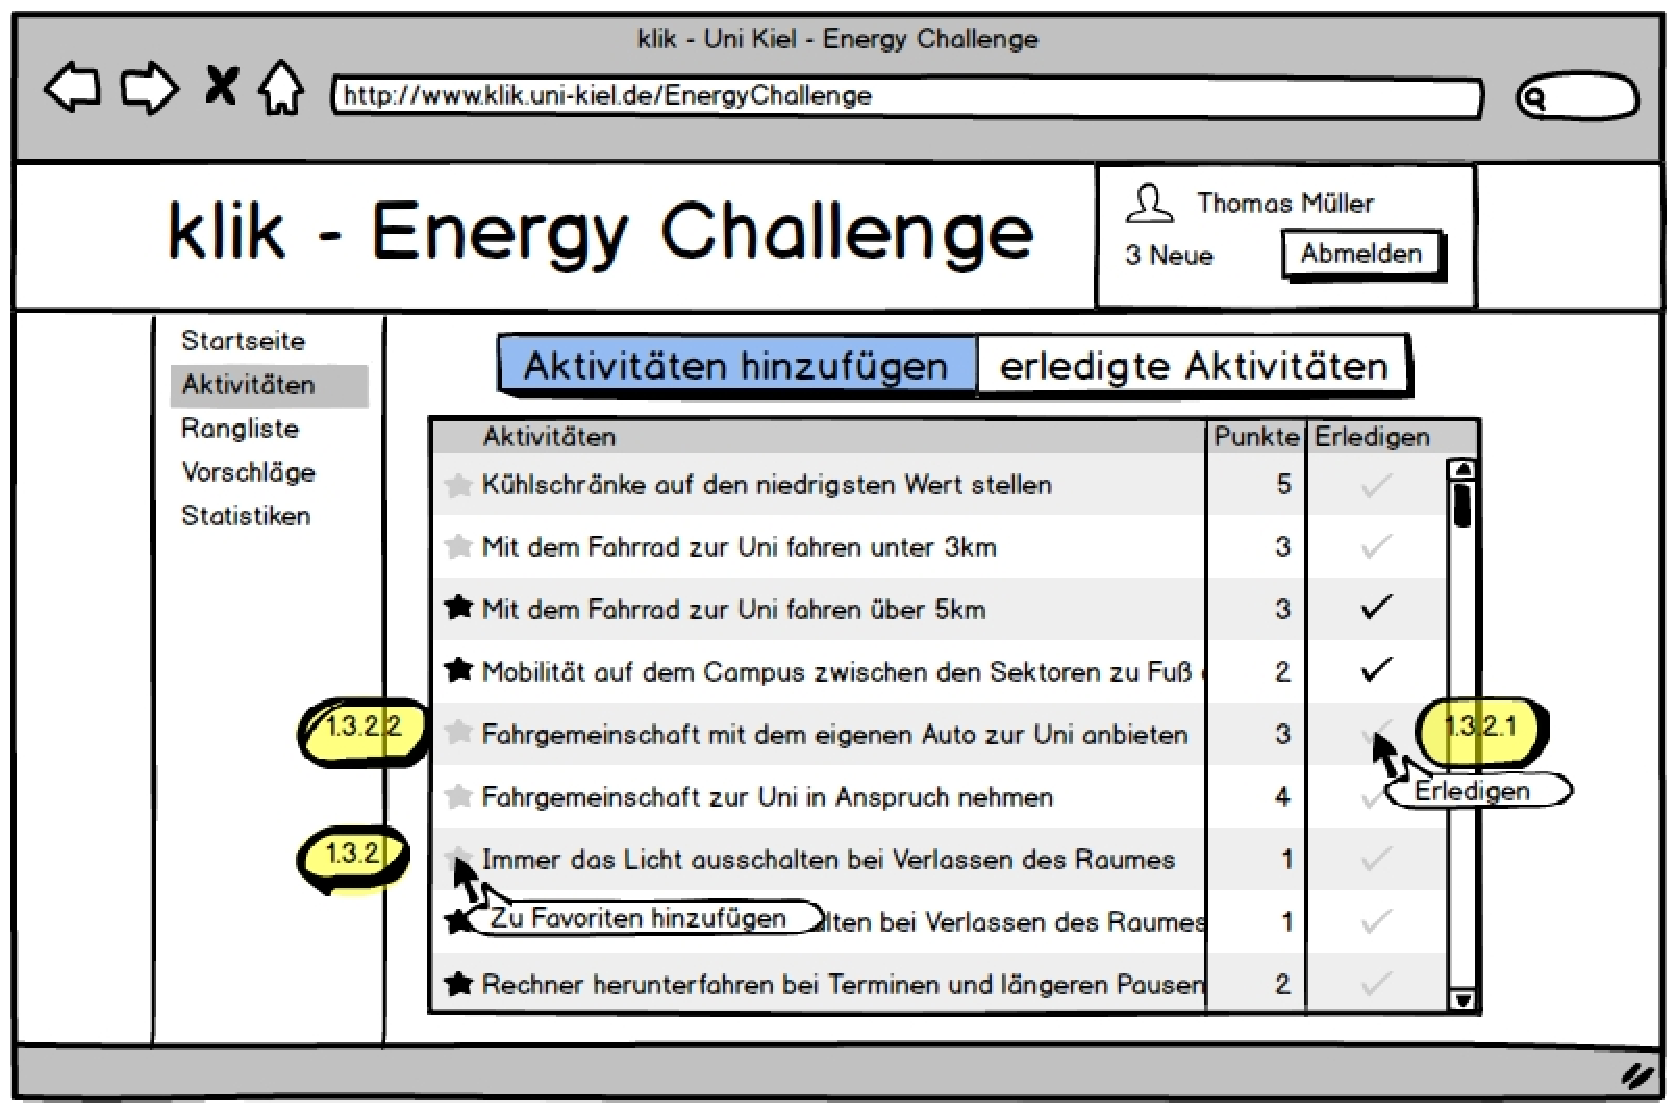
\includegraphics[width=\linewidth]{gfx/mockups/website-aktivitaeten.pdf}
			\caption{Seite zur Verwaltung der eigenen Aktivitäten}
\end{figure}
\begin{figure}[H]
	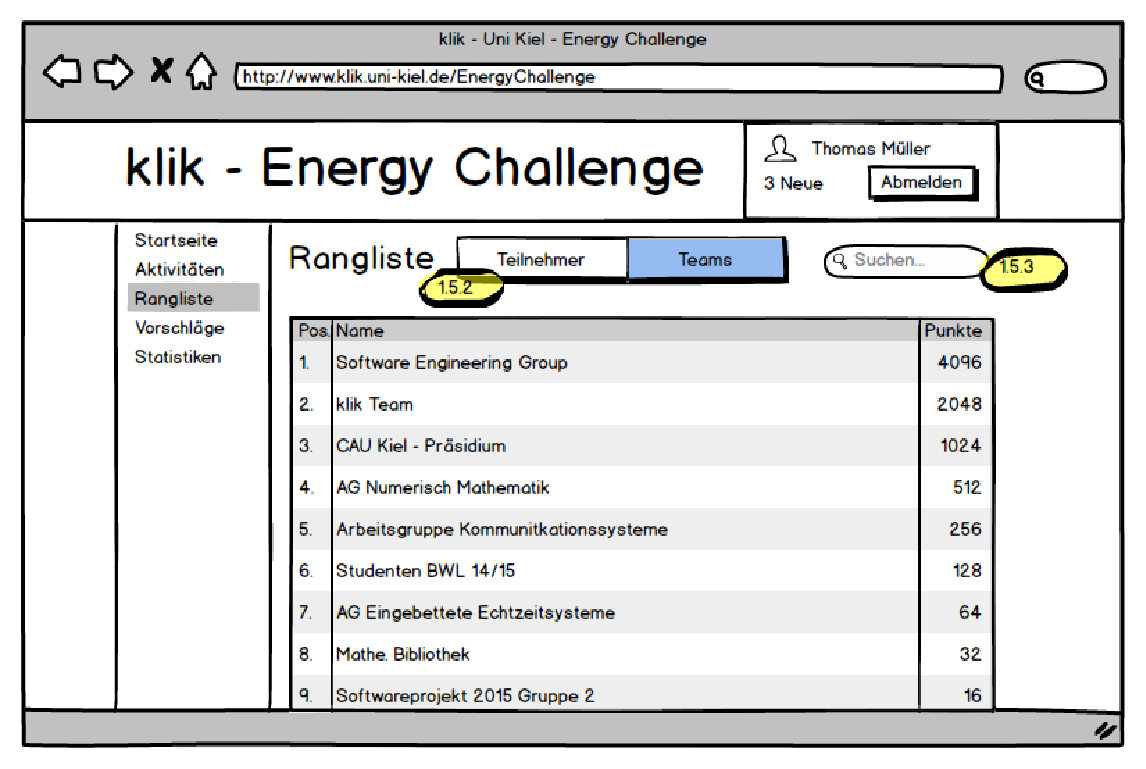
\includegraphics[width=\linewidth]{gfx/mockups/website-rangliste.pdf}
	\caption{Seite mit Übersicht über alle Benutzer/Teams.}
\end{figure}
\begin{figure}[H]
	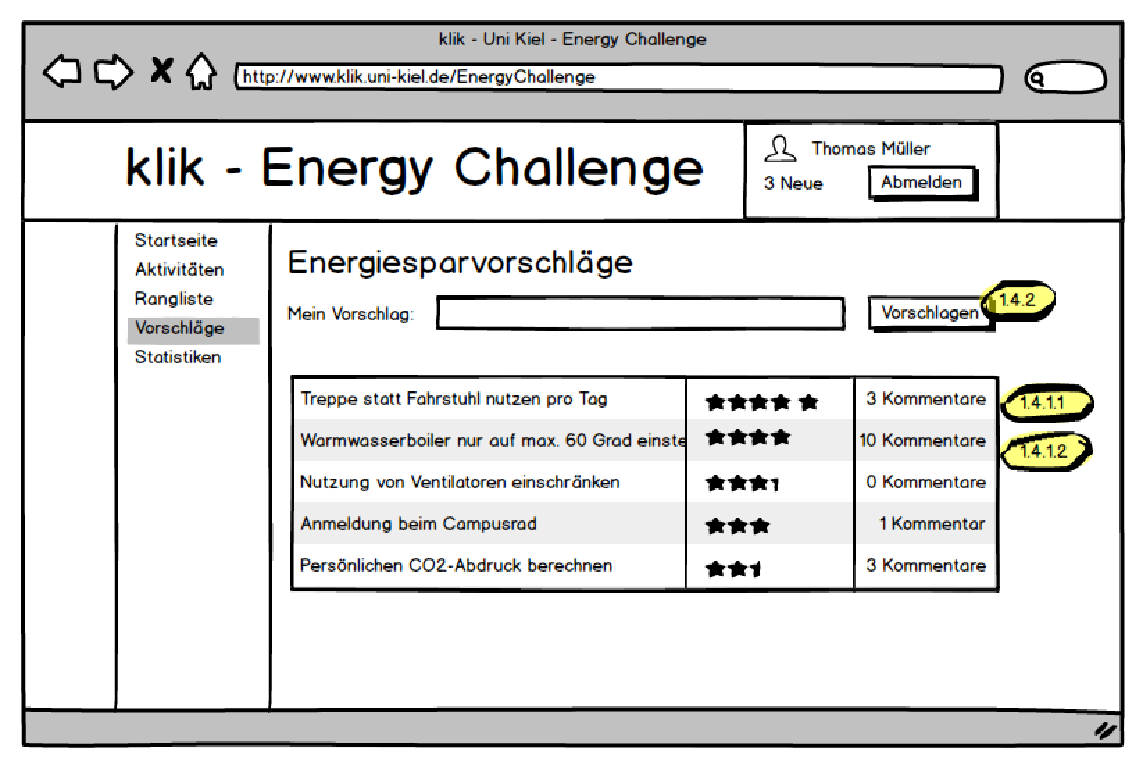
\includegraphics[width=\linewidth]{gfx/mockups/website-vorschlaege.pdf}
		\caption{Seite für die Energiesparvorschläge}
\end{figure}
\begin{figure}[H]
	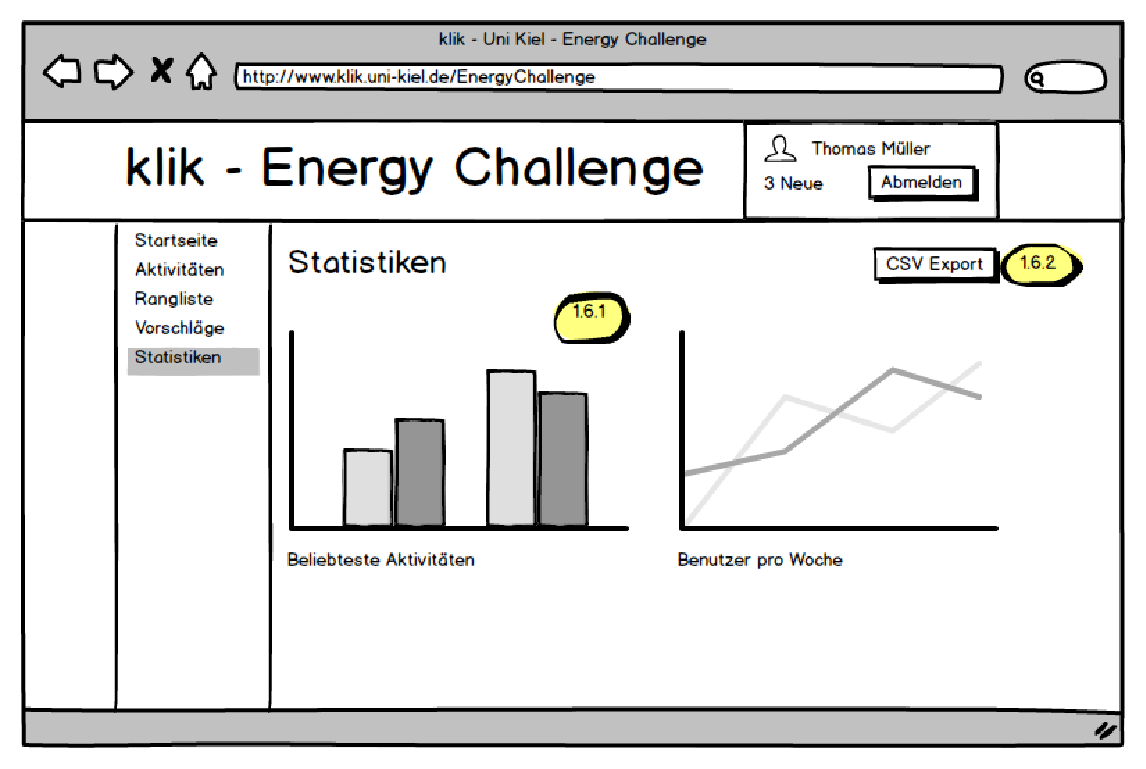
\includegraphics[width=\linewidth]{gfx/mockups/website-statistik.pdf}
	\caption{Seite für die Statistiken}
\end{figure}
\FloatBarrier
\subsection{Android App}
\subsubsection{Grundlegende Anforderungen}
Die Benutzeroberfläche der Android-App soll intuitiv aufgebaut und einfach bedienbar sein. Deshalb
soll die Gestaltung der App den Android-Design-Empfehlungen weitestgehend entsprechen. Die Bedienung
der App erfolgt ausschließlich über einen Touchscreen. \\
Zuerst muss der Benutzer sich in der App anmelden. Nach einer Anmeldung wird ihm eine Startseite angezeigt. Über ein Navigationsmenü soll der Benutzer zwischen den einzelnen Bereichen der App wechseln können, wobei das Navigationsmenü sowohl über eine Schaltfläche als auch über eine Wischgeste vom linken Bildschirmrand aufgerufen werden kann.
\subsubsection{Navigationsstruktur}
\begin{figure}[H]
	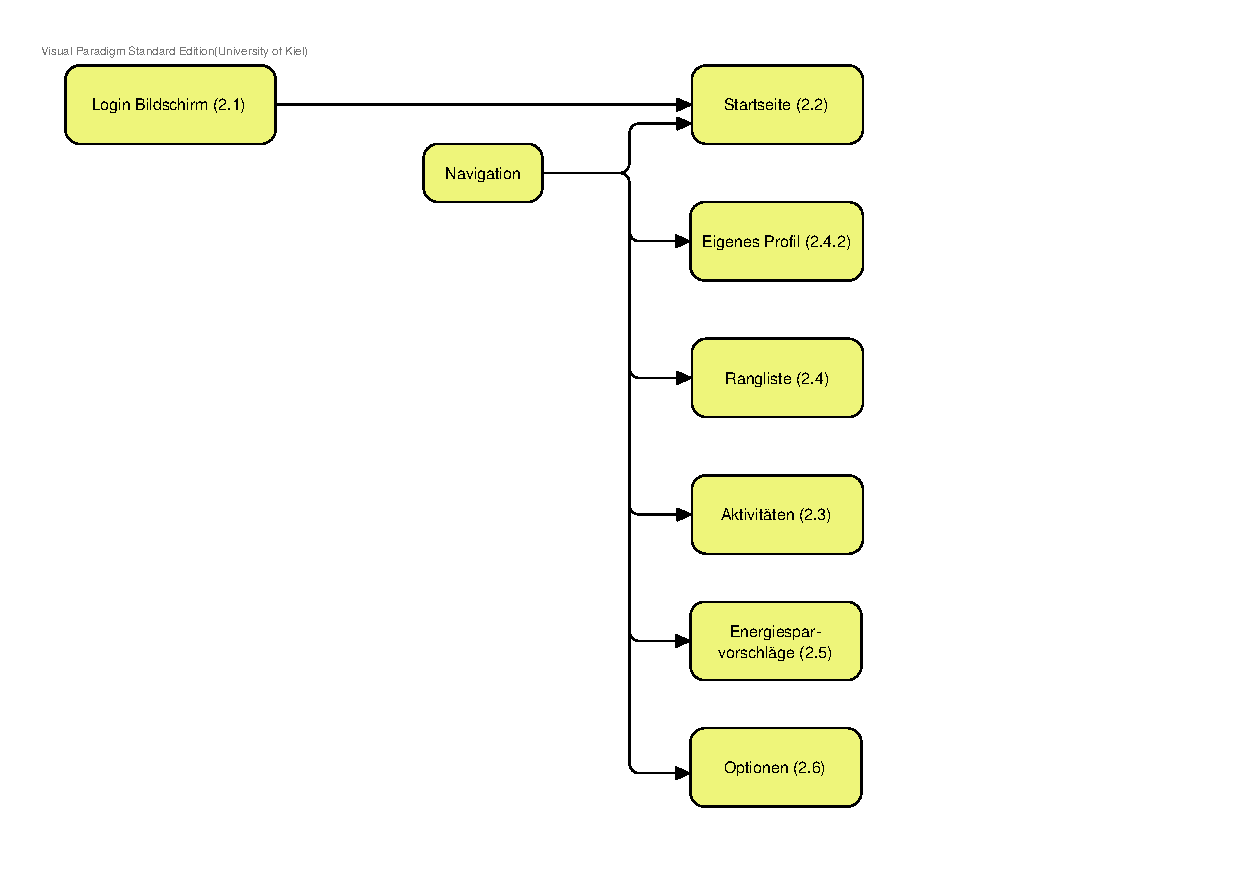
\includegraphics[width=\linewidth]{gfx/guinavigation/GUI-Navigation-App.pdf}
\end{figure}
\subsubsection{GUI-Entwurfsvorschläge}
Die folgenden Grafiken stellen Entwurfsvorschläge für die Benutzeroberfläche dar. Die in gelb eingezeichneten Nummern sind die IDs der Use Cases, die an dieser Stelle verwendet werden.
\begin{figure}[H]
	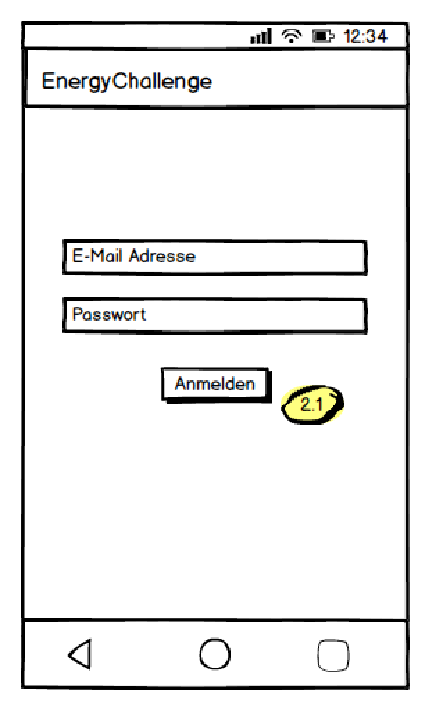
\includegraphics[width=\linewidth]{gfx/mockups/app-login.pdf}
	\caption{Bildschirm zum Anmelden}
\end{figure}
\begin{figure}[H]
	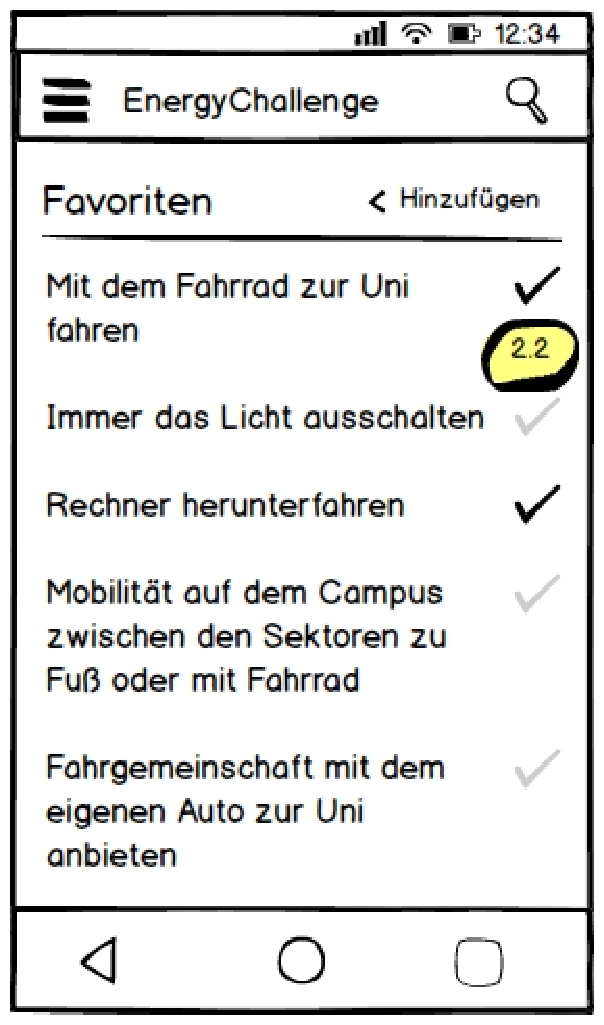
\includegraphics[width=\linewidth]{gfx/mockups/app-main.pdf}
	\caption{Startbildschirm der App}
\end{figure}
\begin{figure}[H]
	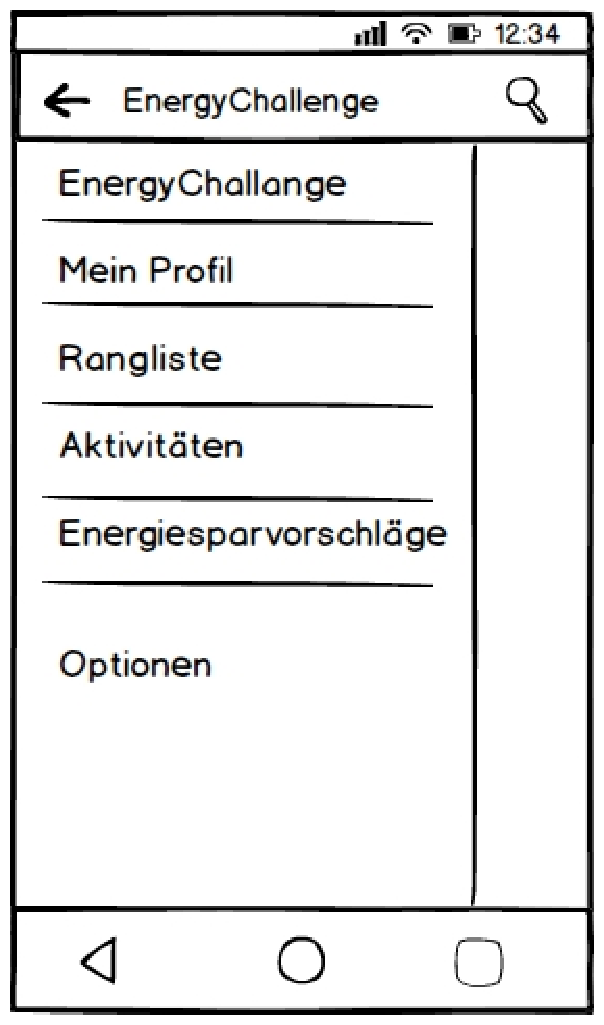
\includegraphics[width=\linewidth]{gfx/mockups/app-navigation.pdf}
	\caption{Navigationsbildschirm der App}
\end{figure}
\begin{figure}[H]
	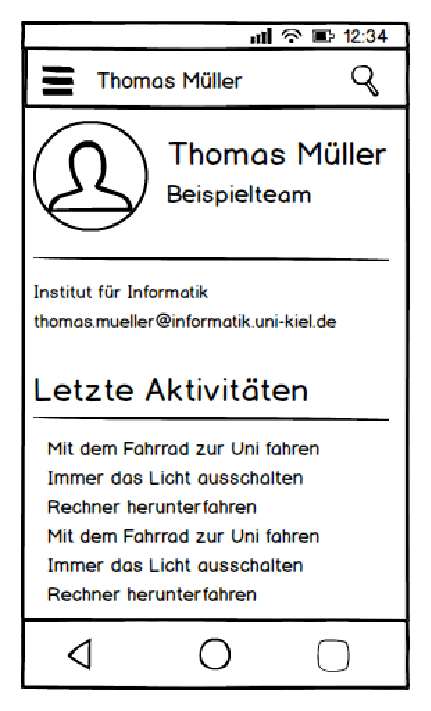
\includegraphics[width=\linewidth]{gfx/mockups/app-meinprofil.pdf}
	\caption{Übersicht über das eigene Profil in der App}
\end{figure}
\begin{figure}[H]
	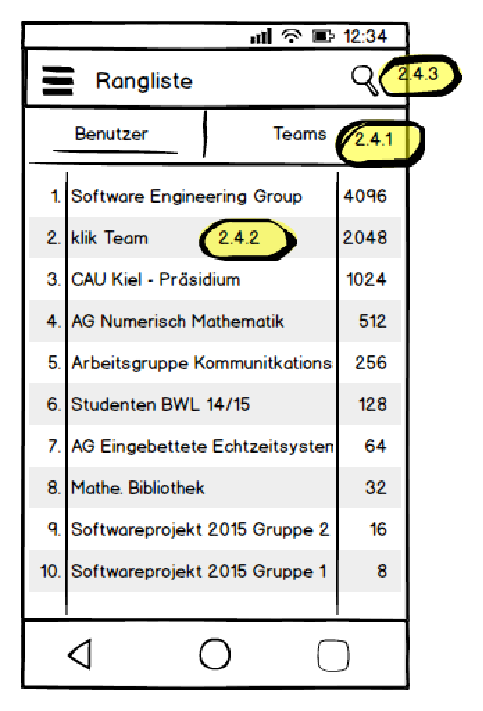
\includegraphics[width=\linewidth]{gfx/mockups/app-rangliste.pdf}
	\caption{Ranglistenansicht in der App}
\end{figure}
\begin{figure}[H]
	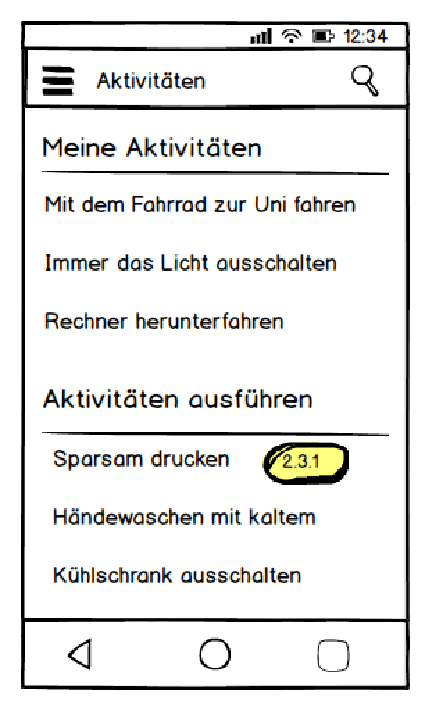
\includegraphics[width=\linewidth]{gfx/mockups/app-aktivitaeten.pdf}
	\caption{Aktivitätenansicht in der App}
\end{figure}
\begin{figure}[H]
	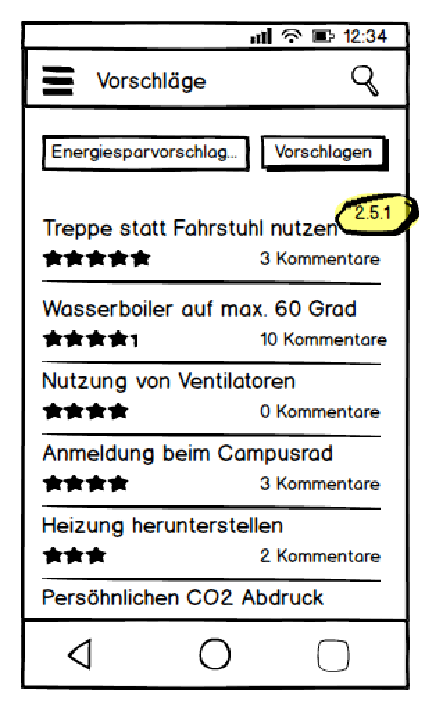
\includegraphics[width=\linewidth]{gfx/mockups/app-vorschlaege.pdf}
	\caption{Energiesparvorschläge in der App}
\end{figure}
\FloatBarrier
%------------------------------------------------
% Qualitaetsanforderung
%------------------------------------------------
\section{Qualitätsanforderung}
\begin{tabular}{|l|c|c|c|c|}
	\hline  & sehr wichtig  & wichtig & weniger wichtig & unwichtig \\ 
	\hline Robustheit  & x &  &  &  \\ 
	\hline Zuverlässigkeit & x &  &  &  \\ 
	\hline Benutzerfreundlichkeit & x &  &  &  \\ 
	\hline Effizienz &  & x &  &  \\ 
	\hline Portierbarkeit  & & x &  &  \\ 
	\hline Kompatibilität & & x &  &  \\ 
	\hline 
\end{tabular} 
\begin{itemize}
\item
Die Produkte des Projekt müssen einen angemessen Namen haben (App-Name, Website-Titel).
\item
Die Produkte sollten eine intuitive, strukturierte und  GUI haben.
\item
Die Android-App und die Website sollte konsistent sein.
\item
Die Produkte sollten leicht zugänglich sein über die Android-App und die Website.
\item
Die Produkte müssen einen schneller Zugriff garantieren.
\item
Die Produkte sollten mit vielen gleichzeitigen Benutzern zurechtkommen.
\end{itemize}


%------------------------------------------------
% Entwicklungsumgebung
%------------------------------------------------
\section{Entwicklungsumgebung}
\subsection{Software}
\begin{itemize}
	\item Java 7 (JDK 1.7)
	\item Eclipse 4.4 mit Grailsplugin
	\item Grails 2.4.4
	\item Visual Paradigm Standard Edition 12
	\item Android Studio 1.1.0
	\item Internetbrowser
\end{itemize}
\subsection{Hardware}
\begin{itemize}
	\item Laptop i5-520m und 4GB RAM oder leistungsst\"arker
\end{itemize}
\subsection{Orgware}
\begin{itemize}
	\item 4 2x1m Writeboard
	\item 1 Flipchart
	\item Beamer und Leinwand
	\item Farbige Karteikarten
\end{itemize}
%------------------------------------------------
% Erganzungen
%------------------------------------------------
\section{Erg\"anzungen}

%------------------------------------------------
% Glossar
%------------------------------------------------
\section{Glossar}

\paragraph{Benutzer} Eine Person, welche sich auf der Projektwebsite registriert hat und über ein Profil verfügt.

\paragraph{Besucher} Eine Person, welche die Projektwebsite im Browser aufruft. Und nicht eingeloggt ist.

\paragraph{Adminbereich} Weboberfläche, über die ein Administrator Verwaltungsaufgaben (z.B. Teilnehmerverwaltung, Aktivitätsverwaltung) ausführen kann.

\paragraph{Android Notification} Eine Benachrichtigung, die über das allgemeine \emph{Notification Center} von Android ausgegeben wird, wo z.B. auch Benachrichtigungen über neue E-Mails, SMS und Termine angezeigt werden.


\end{document}
